\begin{appendices}

\chapter{Job description}
\label{appendix:description}

\begin{figure}[h]
  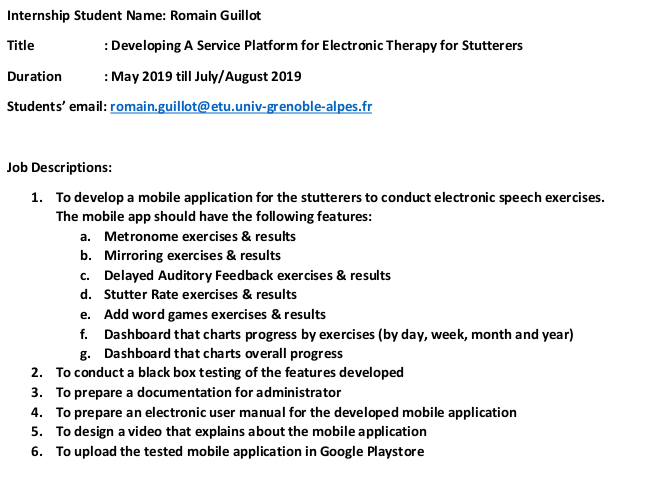
\includegraphics[width=1\linewidth]{content/imgs/description.png}
  \caption*{Job description gave by Dr. Noreen Izza Arshad}
\end{figure}


\begin{landscape}
\chapter{Stutter Manager v3}
\label{appendix:old_app}

\begin{figure}[h]
  \centering
  \begin{subfigure}{.25\textwidth}
    \centering
    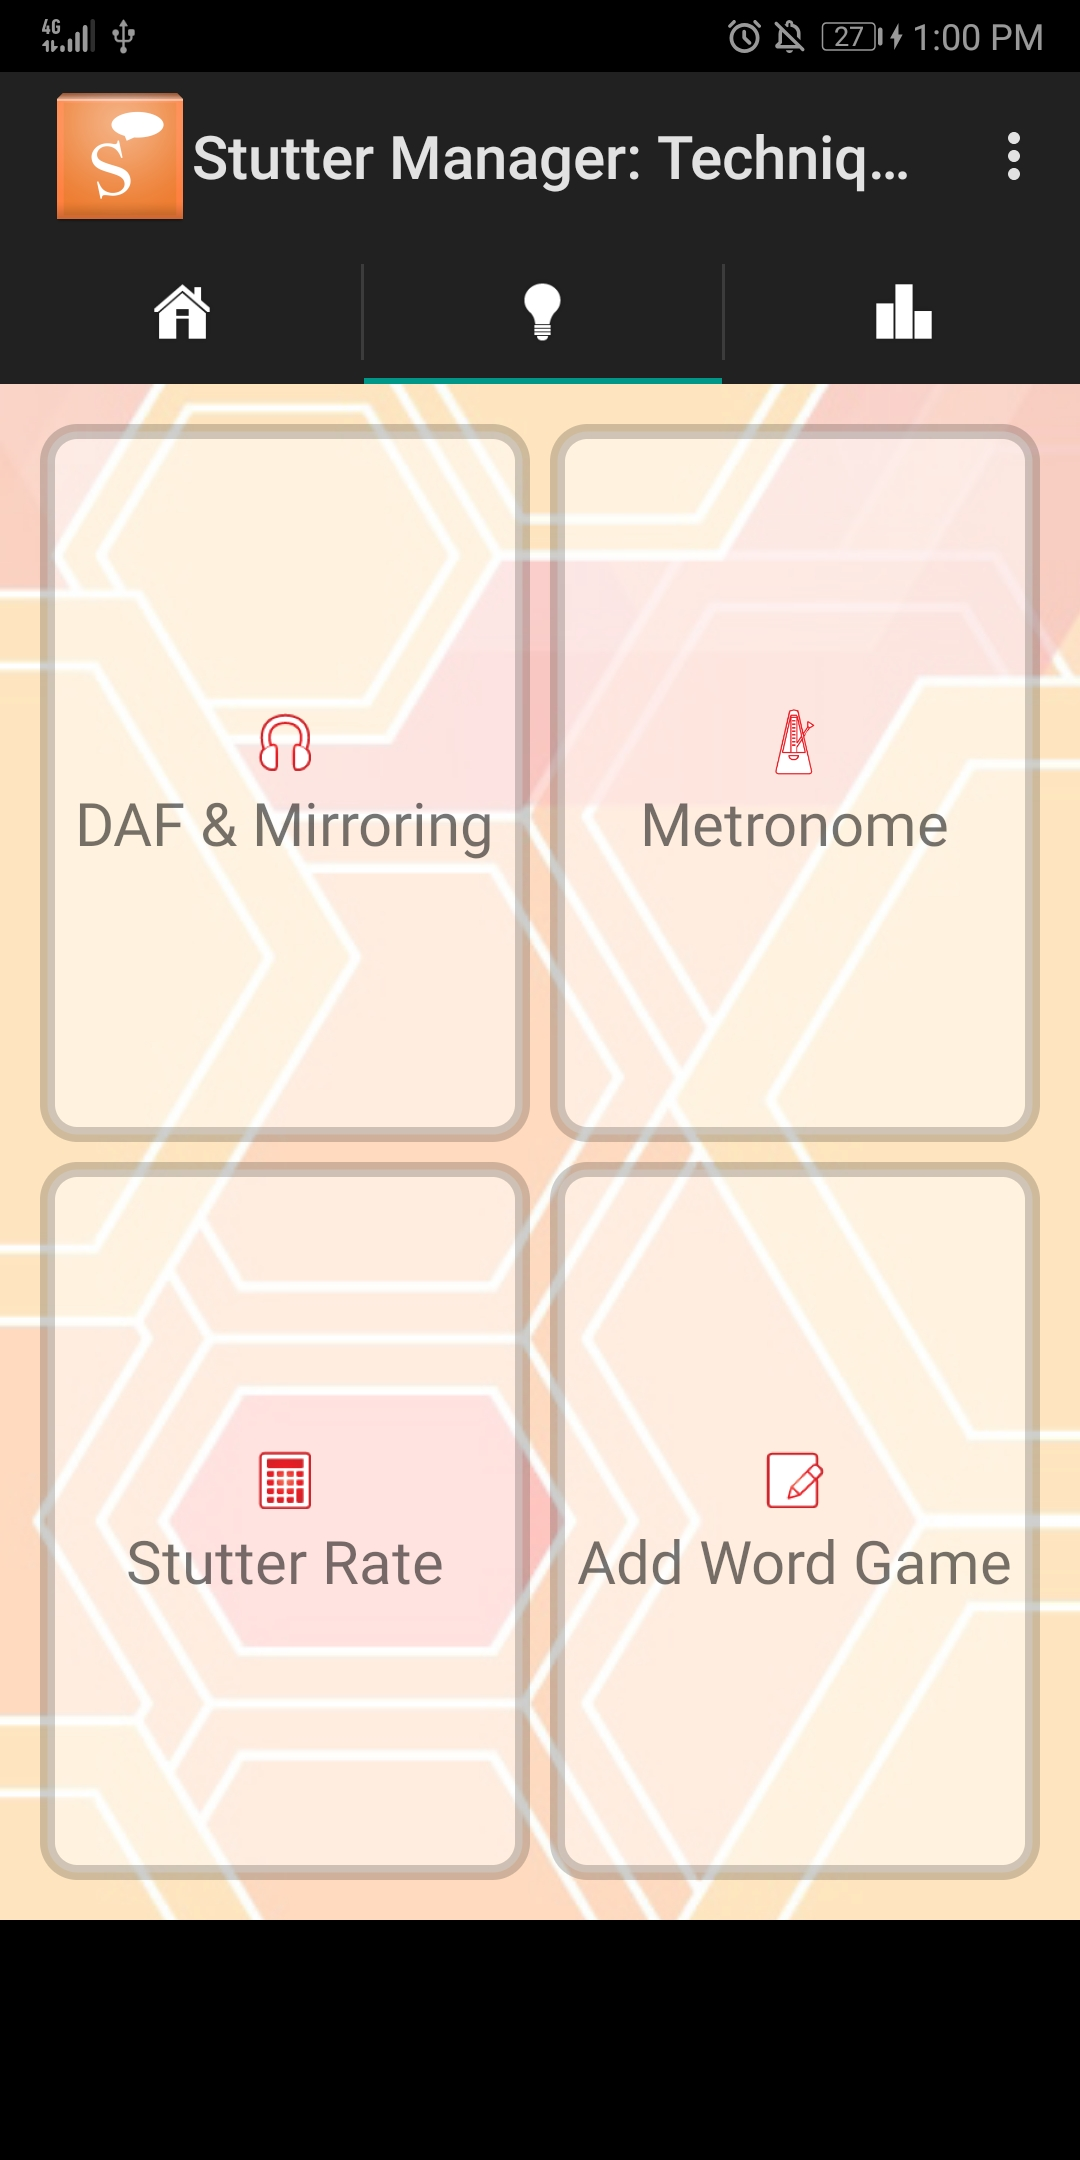
\includegraphics[width=.75\linewidth]{content/imgs/old_app_1.jpg}
    \caption{Homepage}
  \end{subfigure}%
  \begin{subfigure}{.25\textwidth}
    \centering
    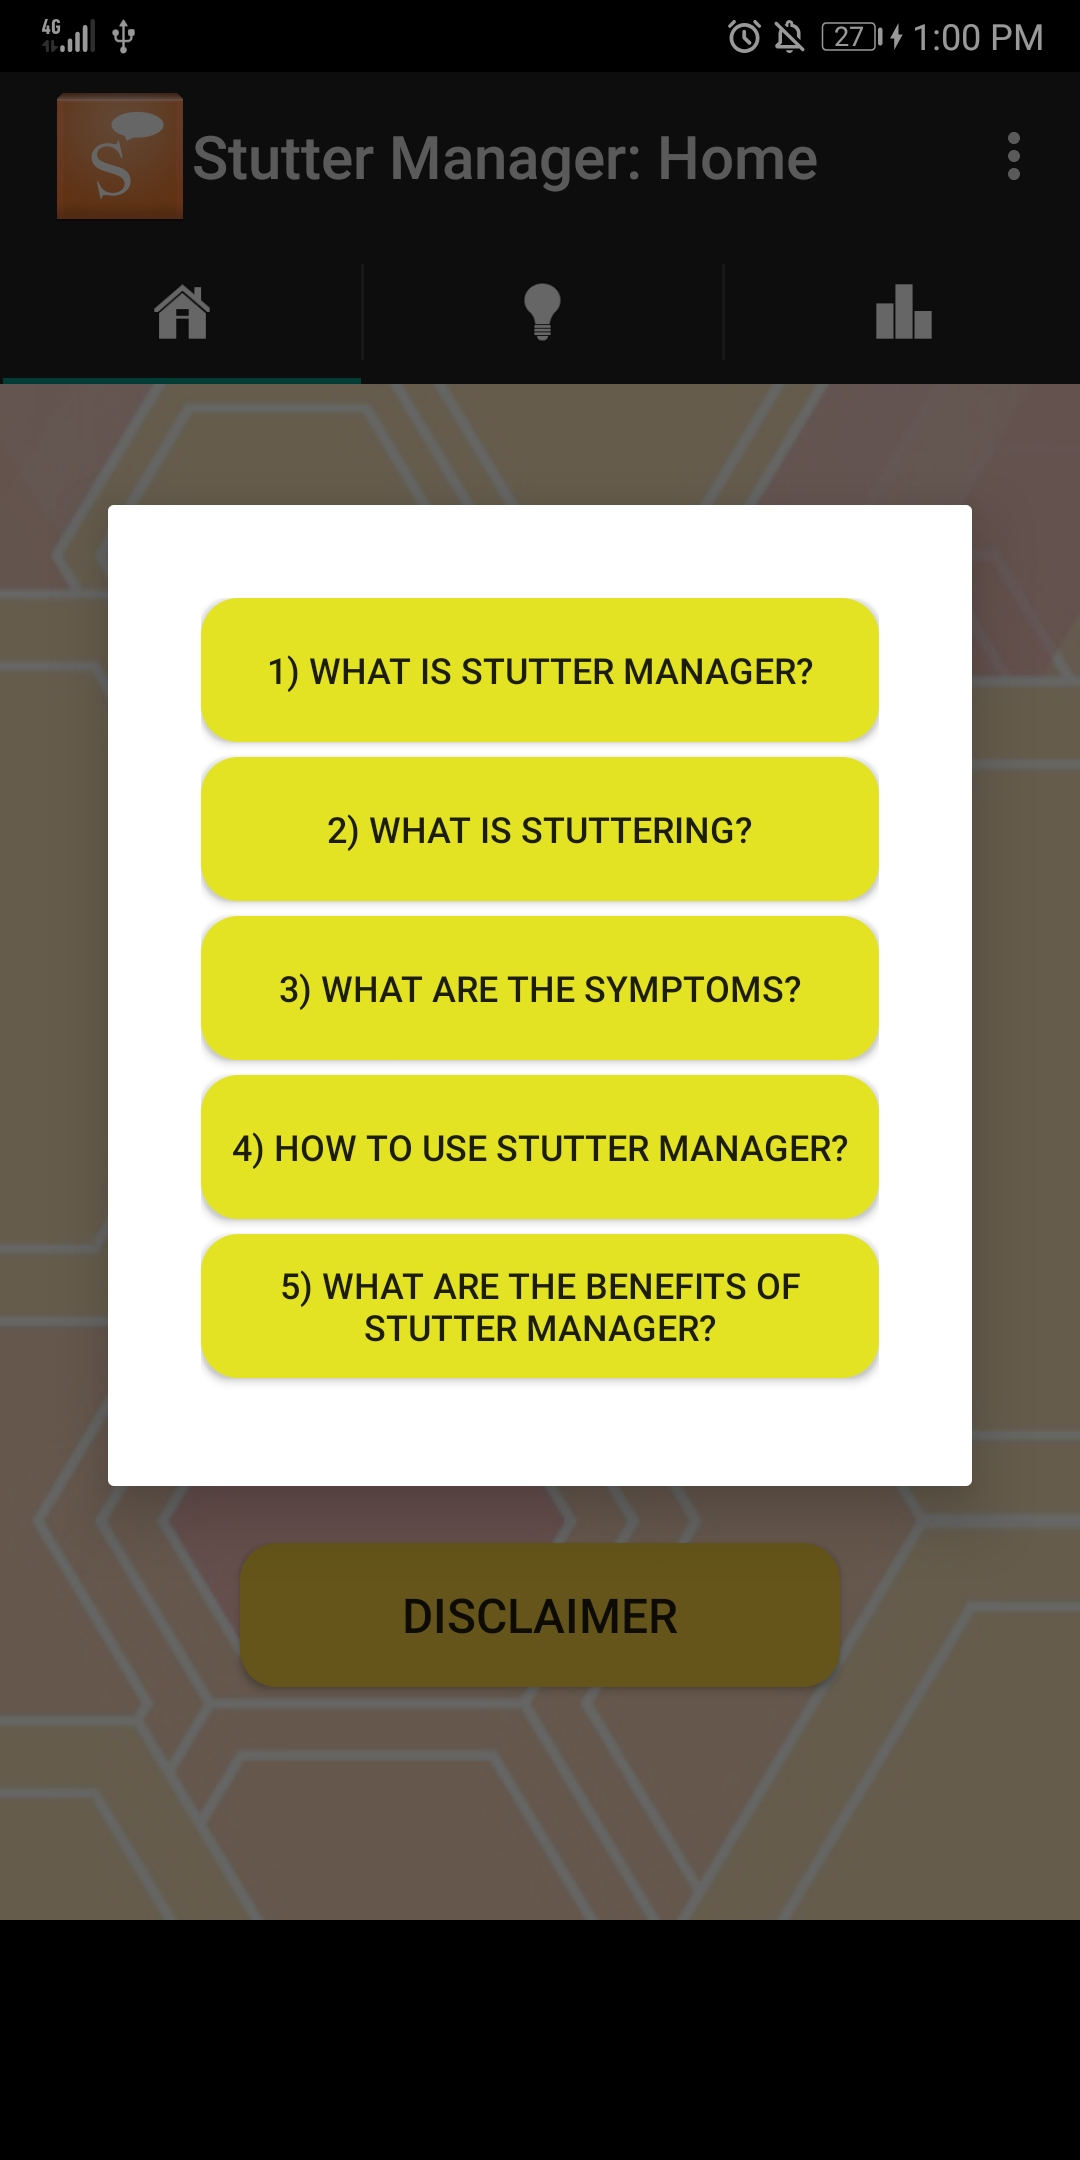
\includegraphics[width=.75\linewidth]{content/imgs/old_app_2.jpg}
    \caption{Information}
  \end{subfigure}%
  \begin{subfigure}{.25\textwidth}
    \centering
    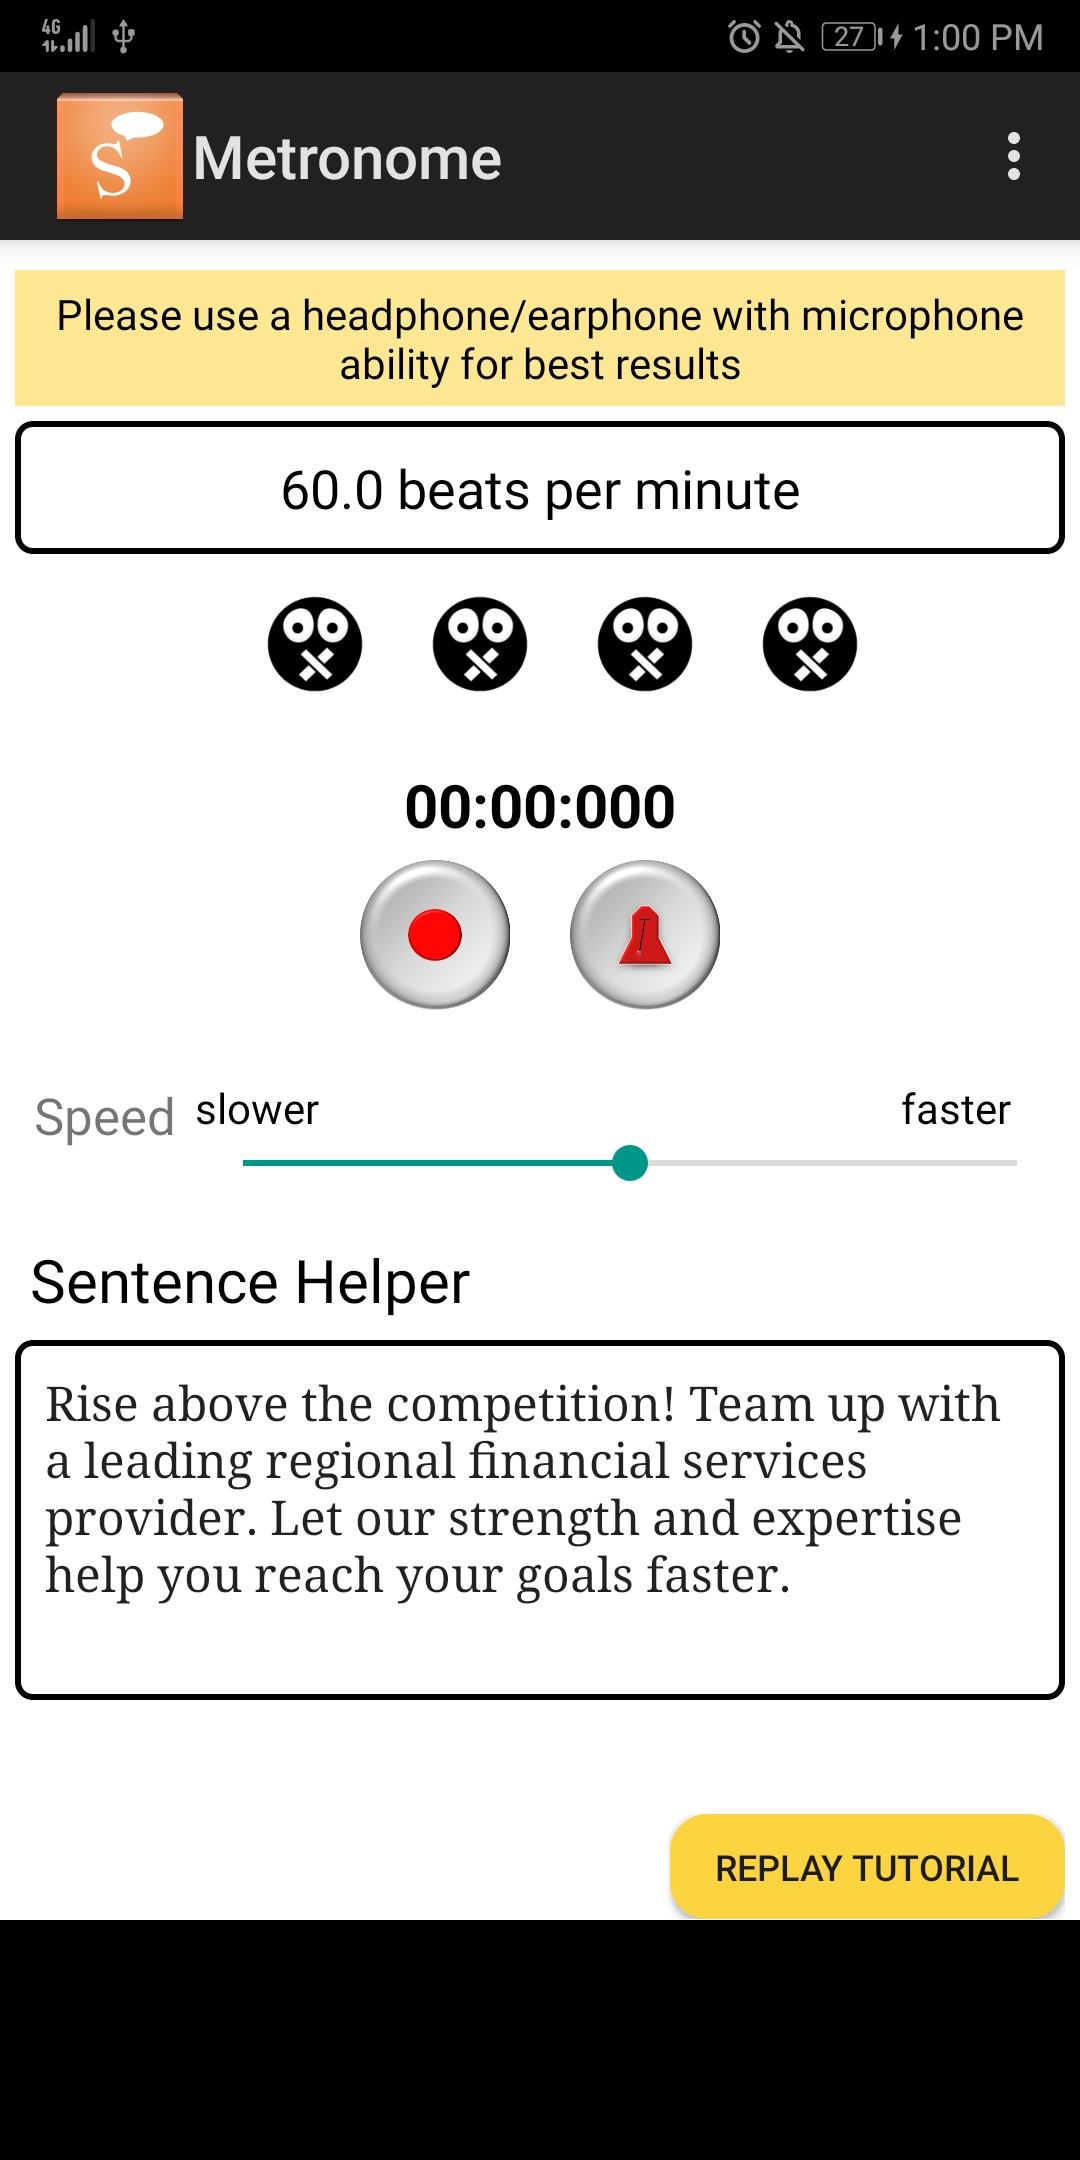
\includegraphics[width=.75\linewidth]{content/imgs/old_app_3.jpg}
    \caption{Exercise : Metronome}
  \end{subfigure}%
  \begin{subfigure}{.25\textwidth}
    \centering
    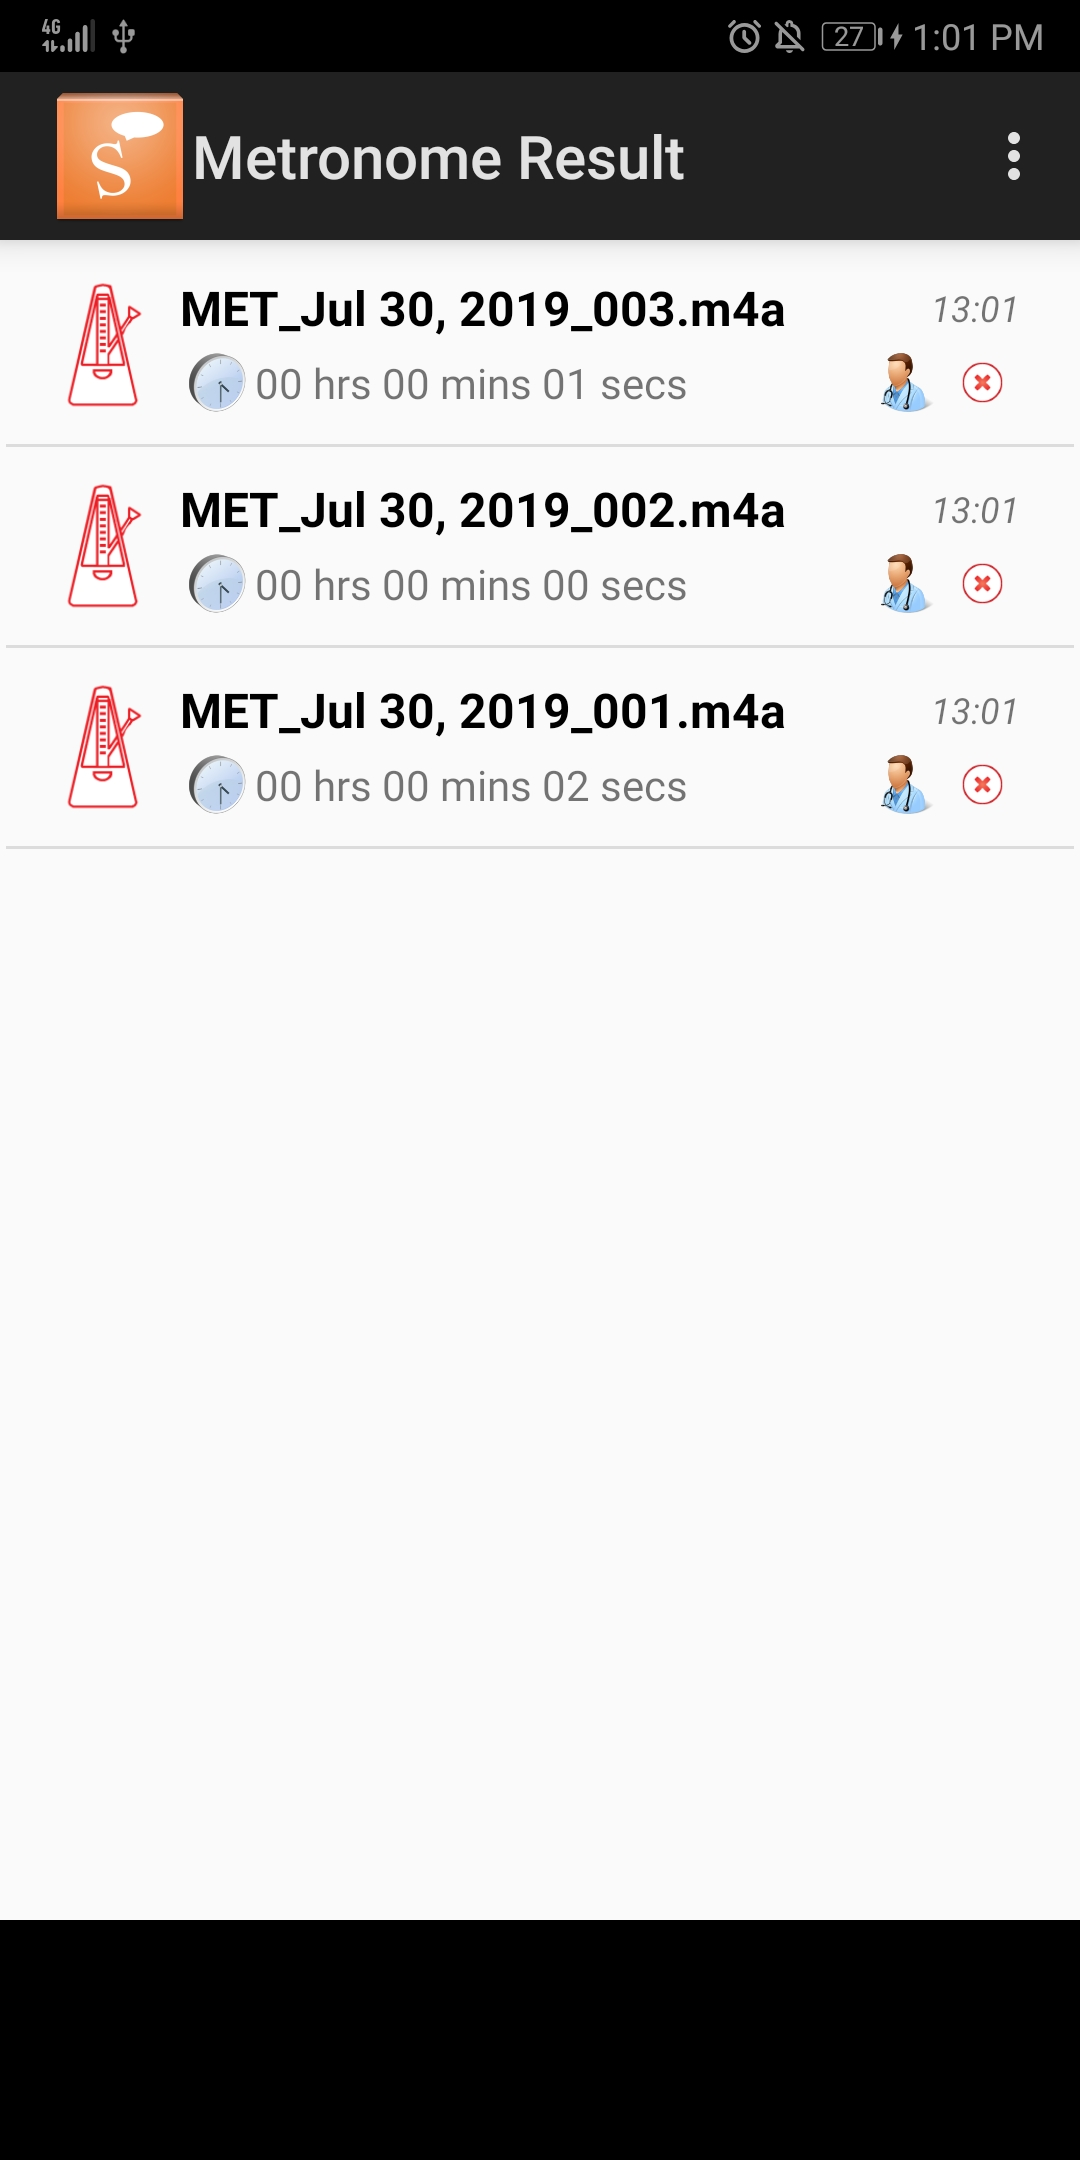
\includegraphics[width=.75\linewidth]{content/imgs/old_app_4.jpg}
    \caption{Progress of the exercise metronome}
  \end{subfigure}
  \caption*{Screenshots of Stutter Manager v3}
\end{figure}

\end{landscape}




\chapter{Comparative study}
\label{appendix:market}
\begin{figure}[h]
  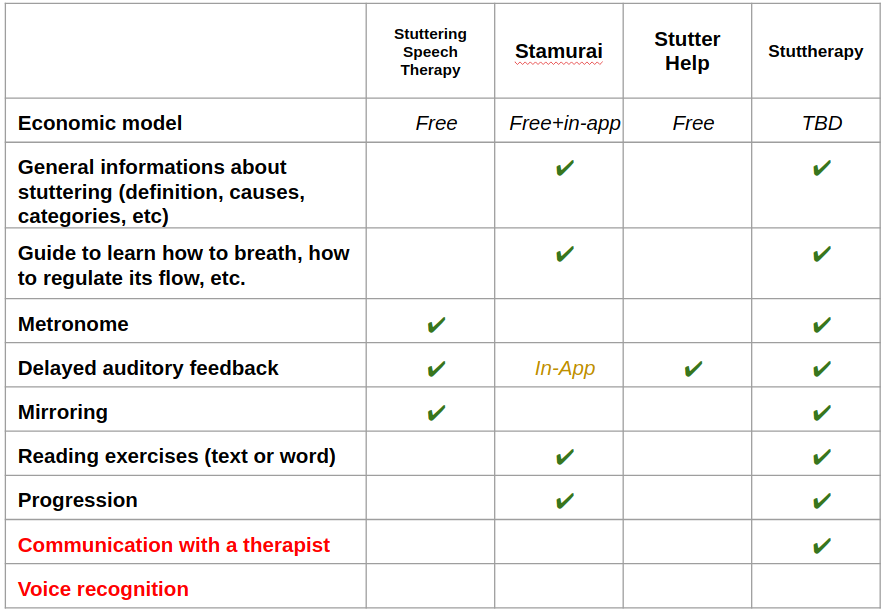
\includegraphics[width=1\linewidth]{content/imgs/market.png}
  \caption*{Comparative study of the applications available on the Play Store in comparison with the functionalities planned for Stuttherapy}
\end{figure}



\chapter{Software requirements specification}
\label{appendix:srs}
\begin{figure}[h]
  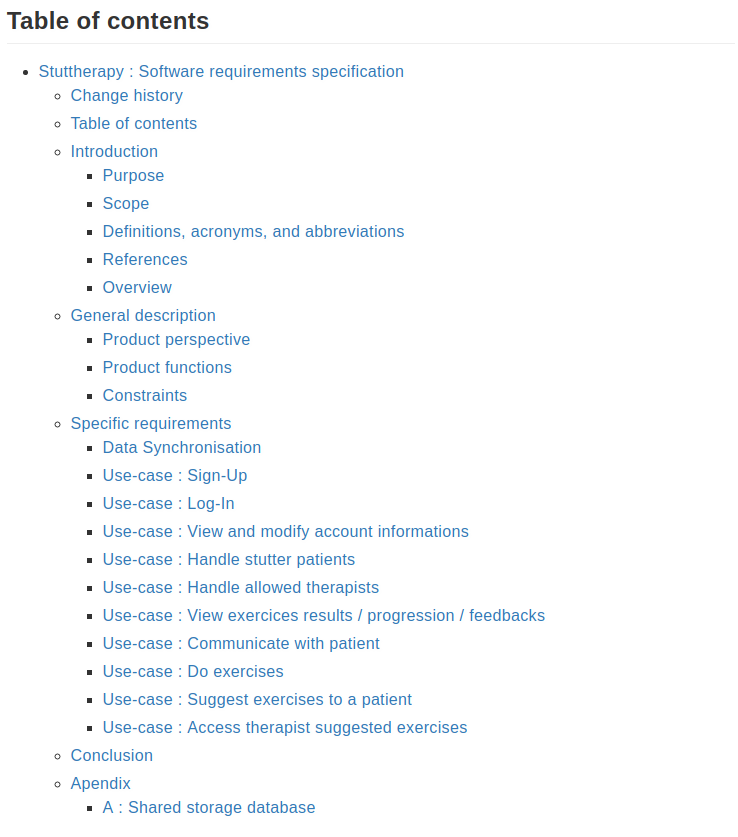
\includegraphics[width=0.7\linewidth]{content/imgs/srs_contents.png}
  \caption*{Table des matières du \textit{Software requirements specification}}
\end{figure}

\begin{displayquote}
The software requirements specification lays out functional and non-functional requirements, and it may include a set of use cases that describe user interactions that the software must provide to the user for perfect interaction.
\end{displayquote}
\hspace*{\fill} \textit{Wikipedia - Software Requirements Specification}



\chapter{Software requirements specifications - Use case example}
\label{appendix:srs_example}
\begin{figure}[h]
  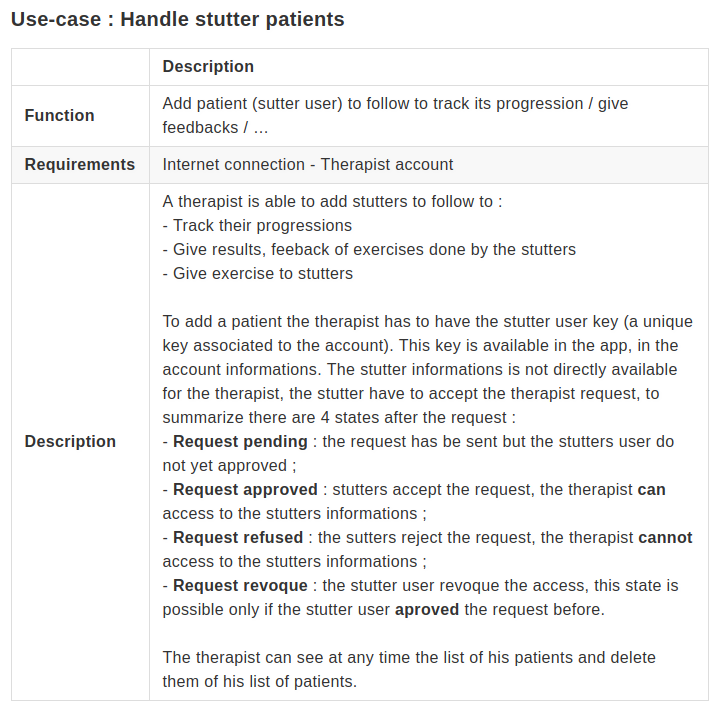
\includegraphics[width=1\linewidth]{content/imgs/srs_use_case_ex.png}
  \caption*{Specification of the use case \textbf{Handle stutter patients}}
\end{figure}




\begin{landscape}
  \label{appendix:gantt}
  \chapter{Forecast Gantt chart}
  \begin{figure}[H]
    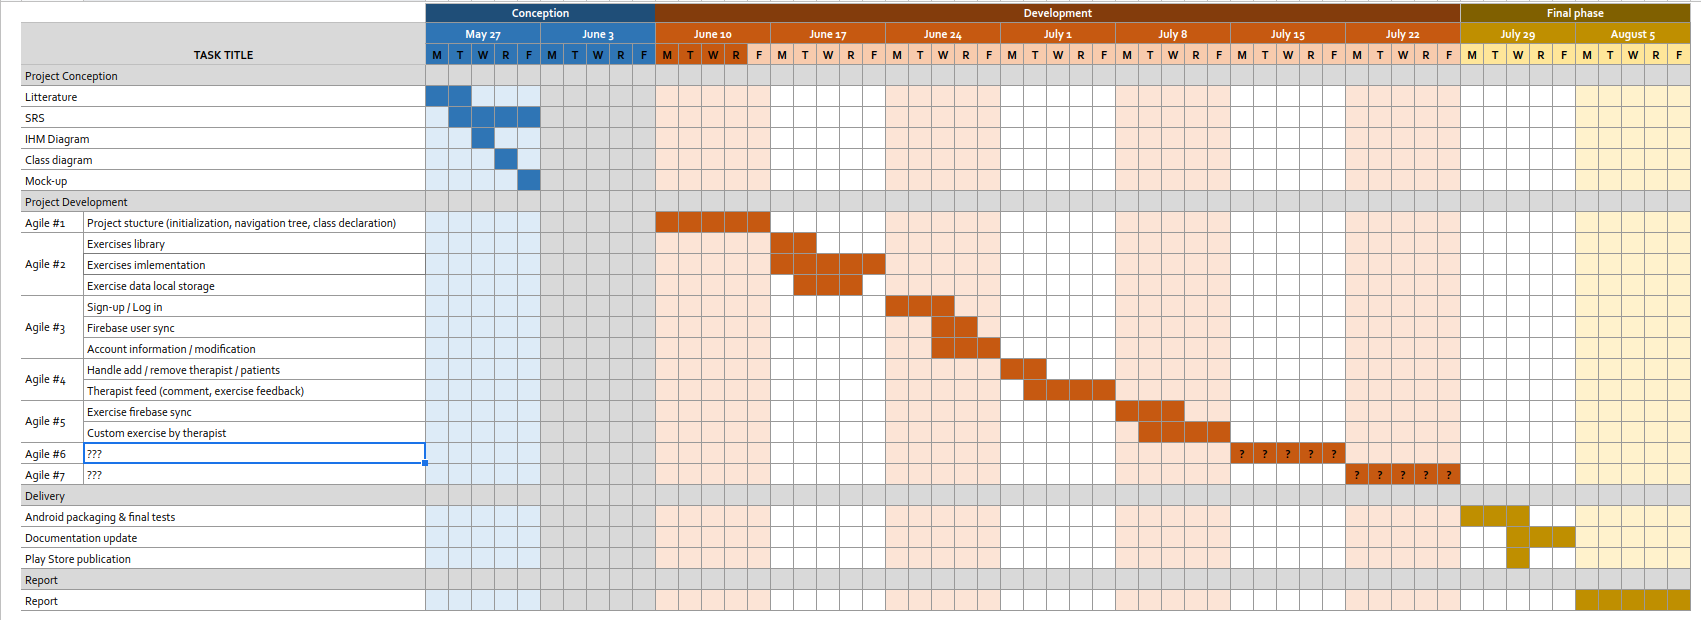
\includegraphics[width=1\linewidth]{content/imgs/gantt.png}
    \caption*{Forecast Gantt chart}
  \end{figure}
\end{landscape}


\chapter{Release Github}
\label{appendix:release}
\begin{figure}[H]
  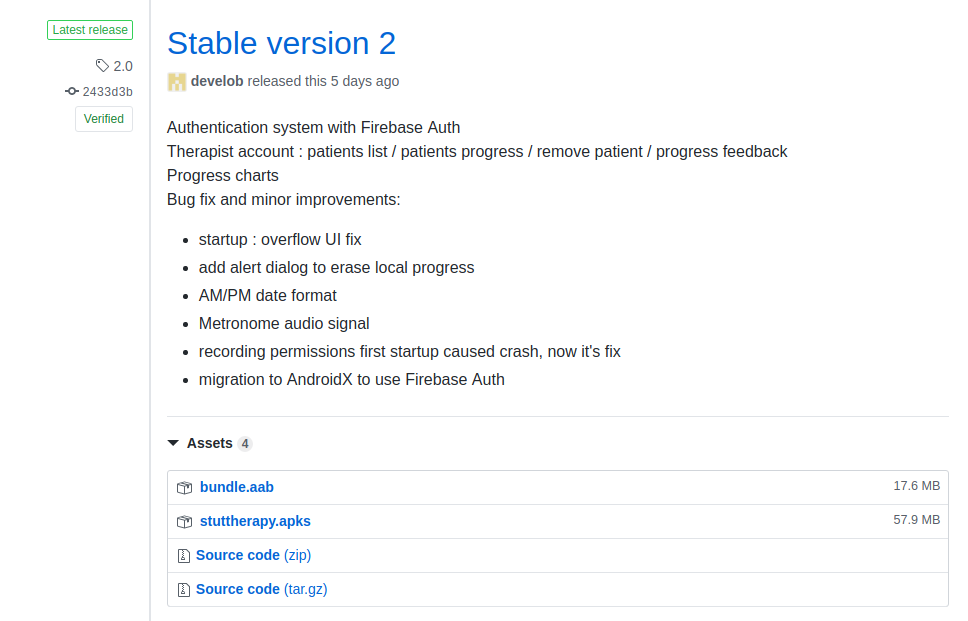
\includegraphics[width=1\linewidth]{content/imgs/release_ex.png}
  \caption*{Finale release}
\end{figure}

\chapter{GUI diagram}
\label{appendix:ihm}
\begin{figure}[H]
  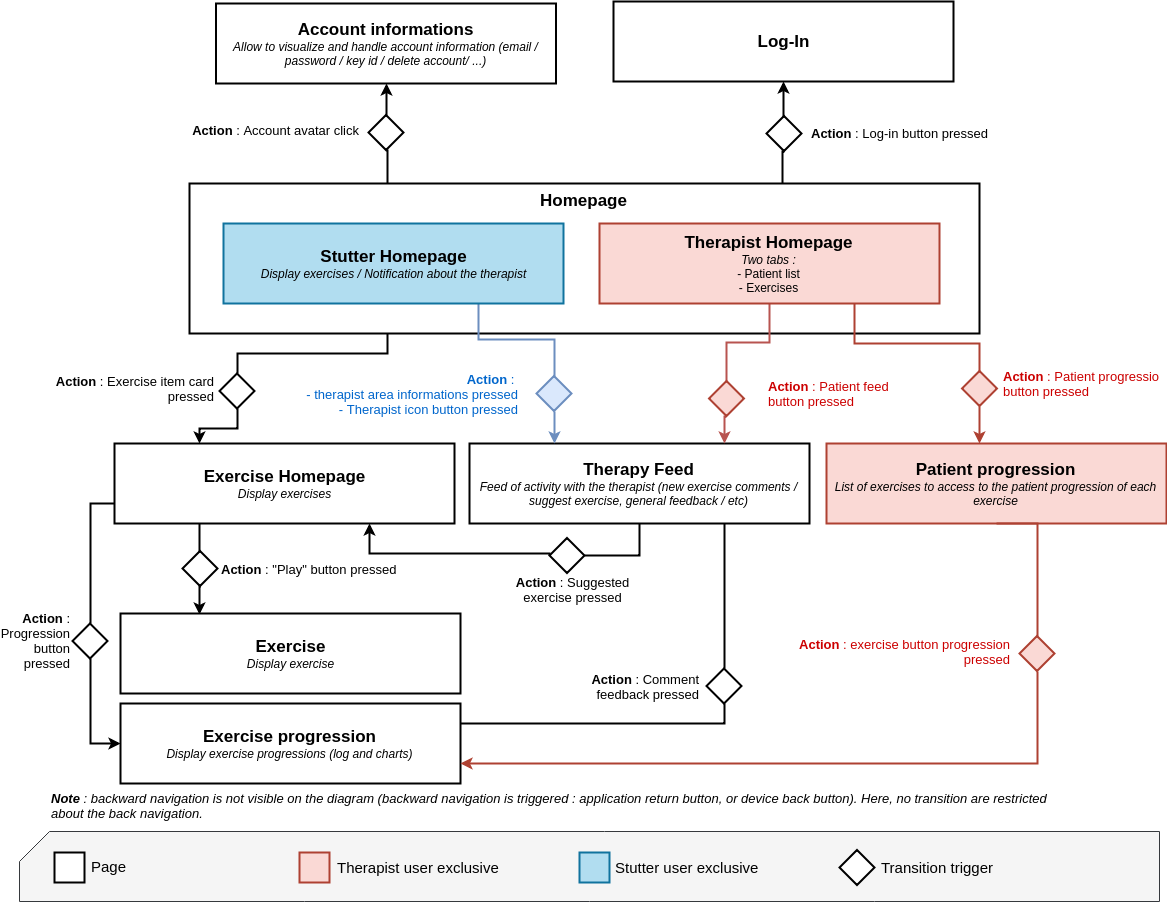
\includegraphics[width=1\linewidth]{content/imgs/IHM_diagram.png}
  \caption*{GUI diagram}
\end{figure}


\chapter{Wireframes}
\label{appendix:wireframes}
\section{Page principales}
\begin{figure}[H]
  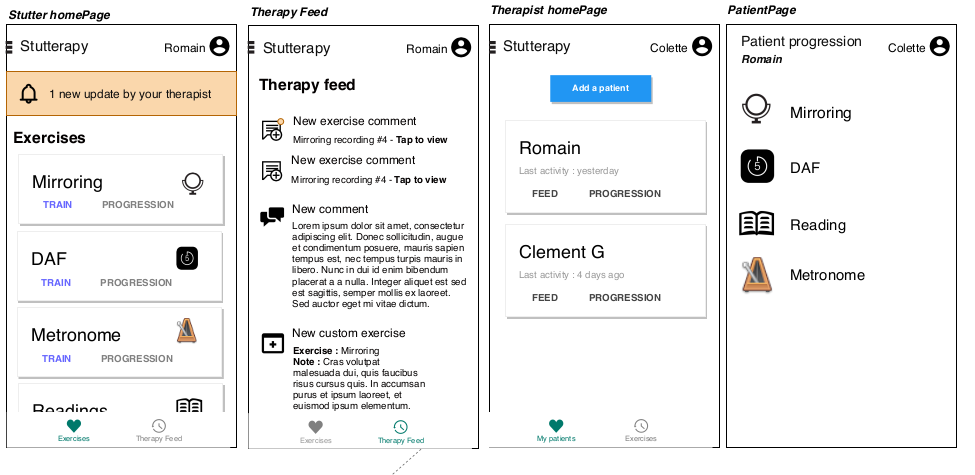
\includegraphics[width=1\linewidth]{content/imgs/maquette1.png}
\end{figure}

\section{Exercises}
\begin{figure}[H]
  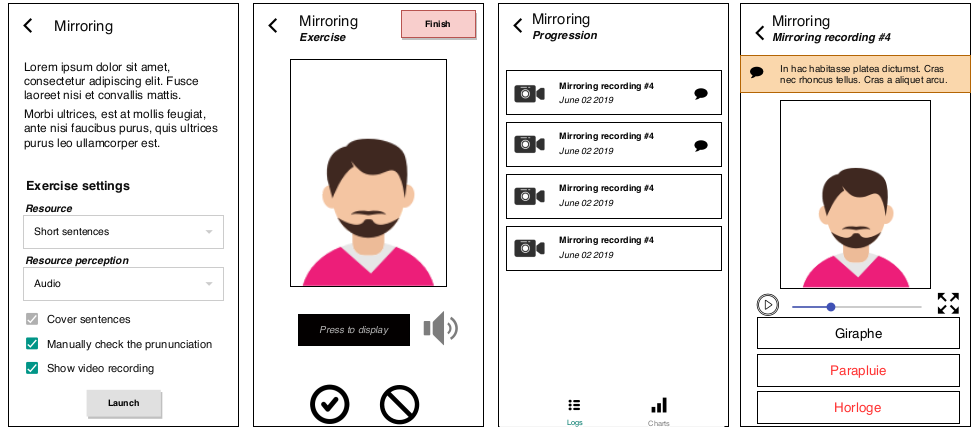
\includegraphics[width=1\linewidth]{content/imgs/maquette2a.png}
  \caption*{Exercise : Mirroring}
\end{figure}

\begin{figure}[H]
  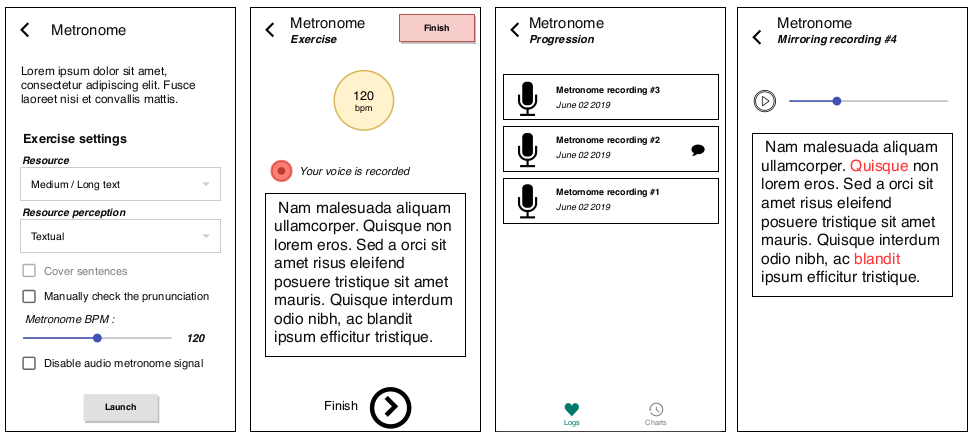
\includegraphics[width=1\linewidth]{content/imgs/maquette2b.png}
  \caption*{Exercise : Metronome}
\end{figure}

\begin{figure}[H]
  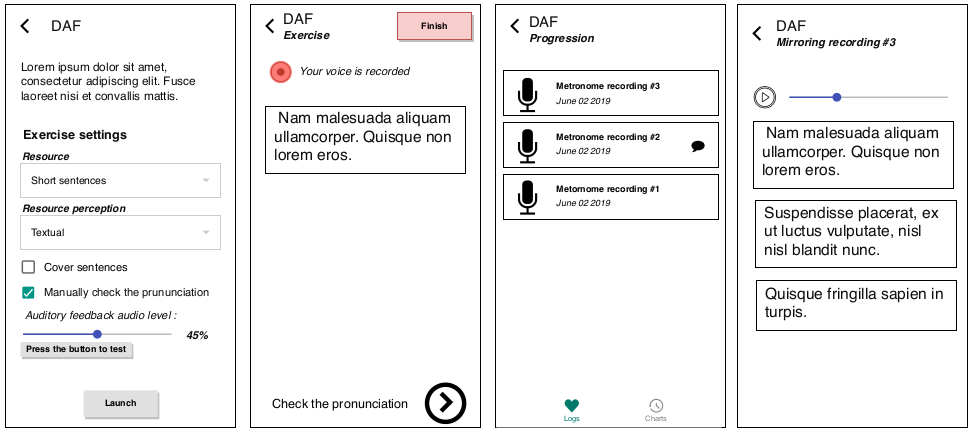
\includegraphics[width=1\linewidth]{content/imgs/maquette2c.png}
  \caption*{Exercise : DAF (delayed auditory feedback)}
\end{figure}

\begin{figure}[H]
  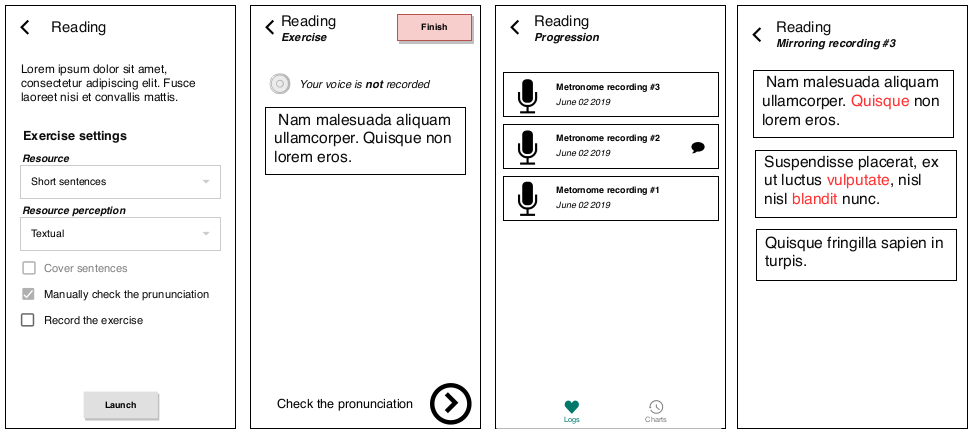
\includegraphics[width=1\linewidth]{content/imgs/maquette2d.png}
  \caption*{Exercise : Reading}
\end{figure}

\section{Divers}
\begin{figure}[H]
  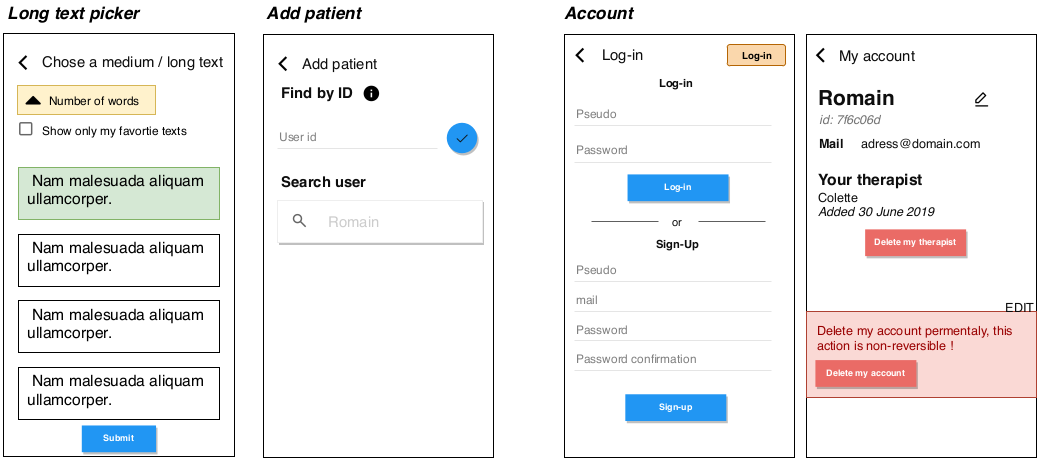
\includegraphics[width=1\linewidth]{content/imgs/maquette3.png}
  \caption*{Text selector / adding a patient / account information}
\end{figure}






\begin{landscape}
\chapter{Class diagram}
\label{appendix:class}
\vspace{-35pt}
\begin{figure}[H]
  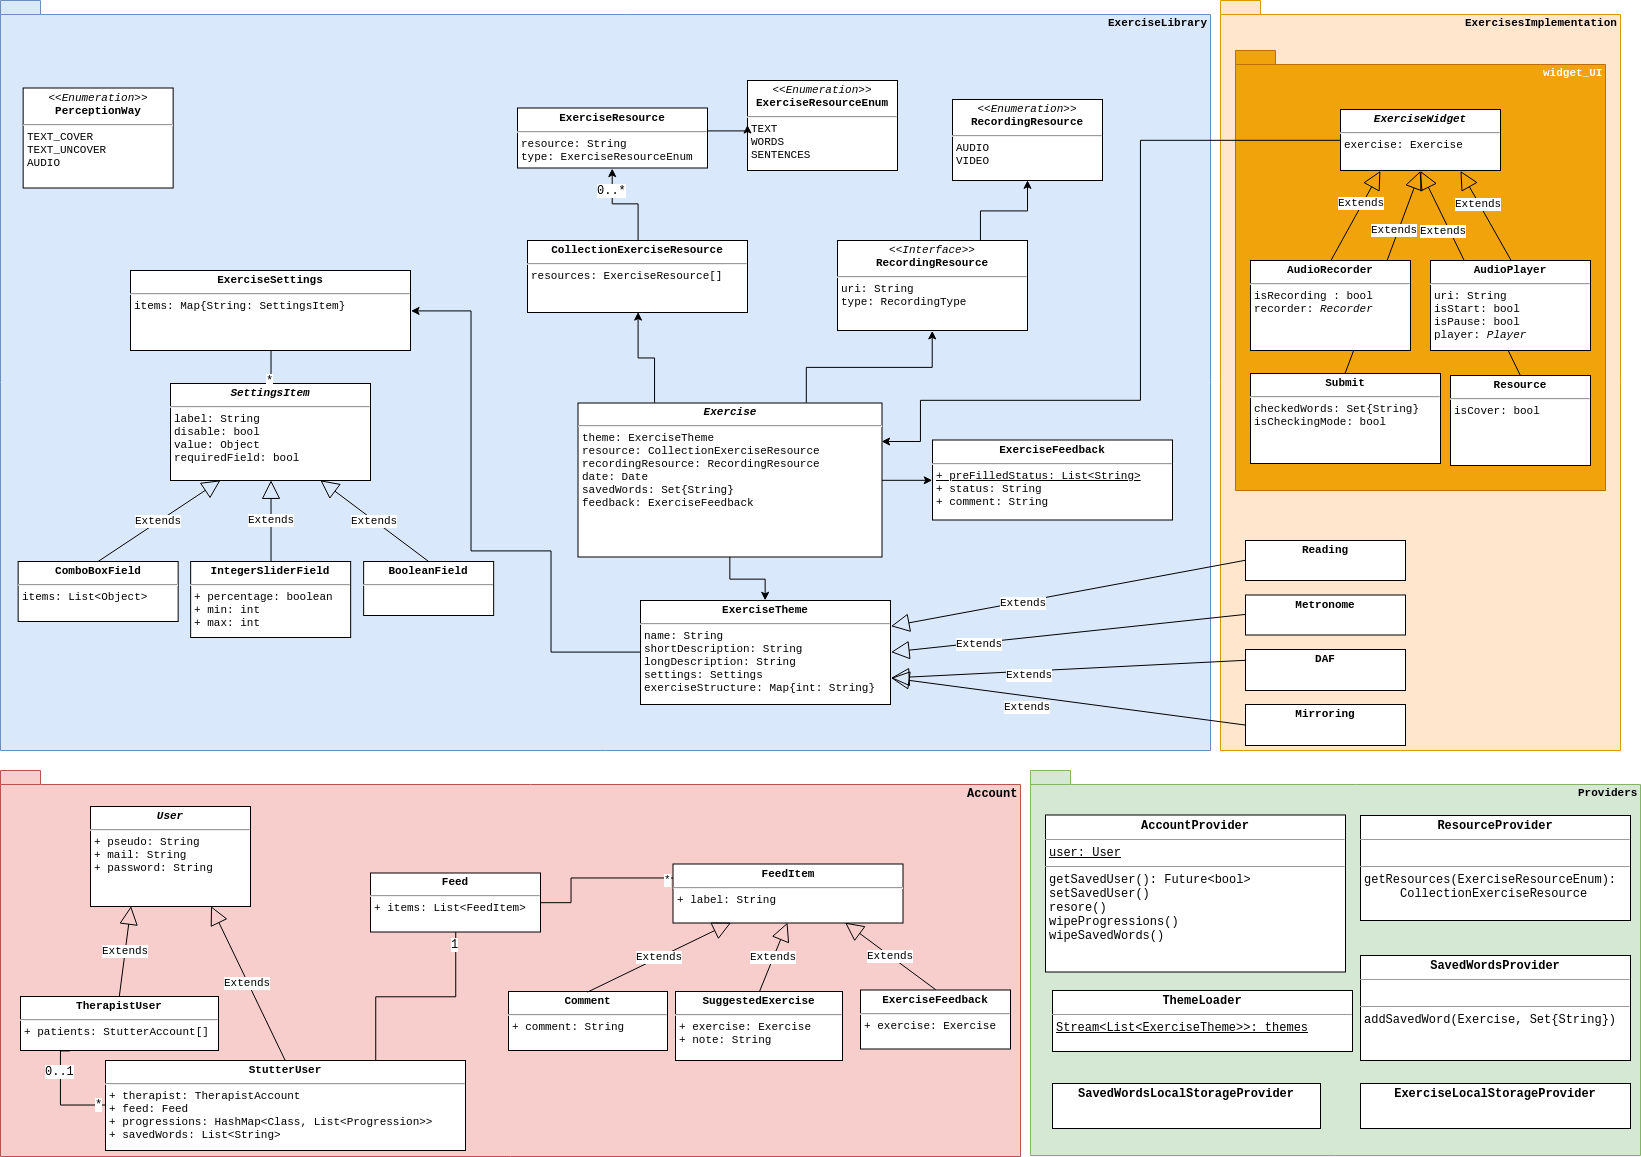
\includegraphics[width=0.9\linewidth]{content/imgs/app_class_diagram.png}
  \caption*{Class diagram}
\end{figure}
\end{landscape}


\begin{landscape}
\chapter{Stuttherapy - Screenshots}
\label{appendix:screenshots}

\begin{figure}[h]
  \centering
  \begin{subfigure}{.25\textwidth}
    \centering
    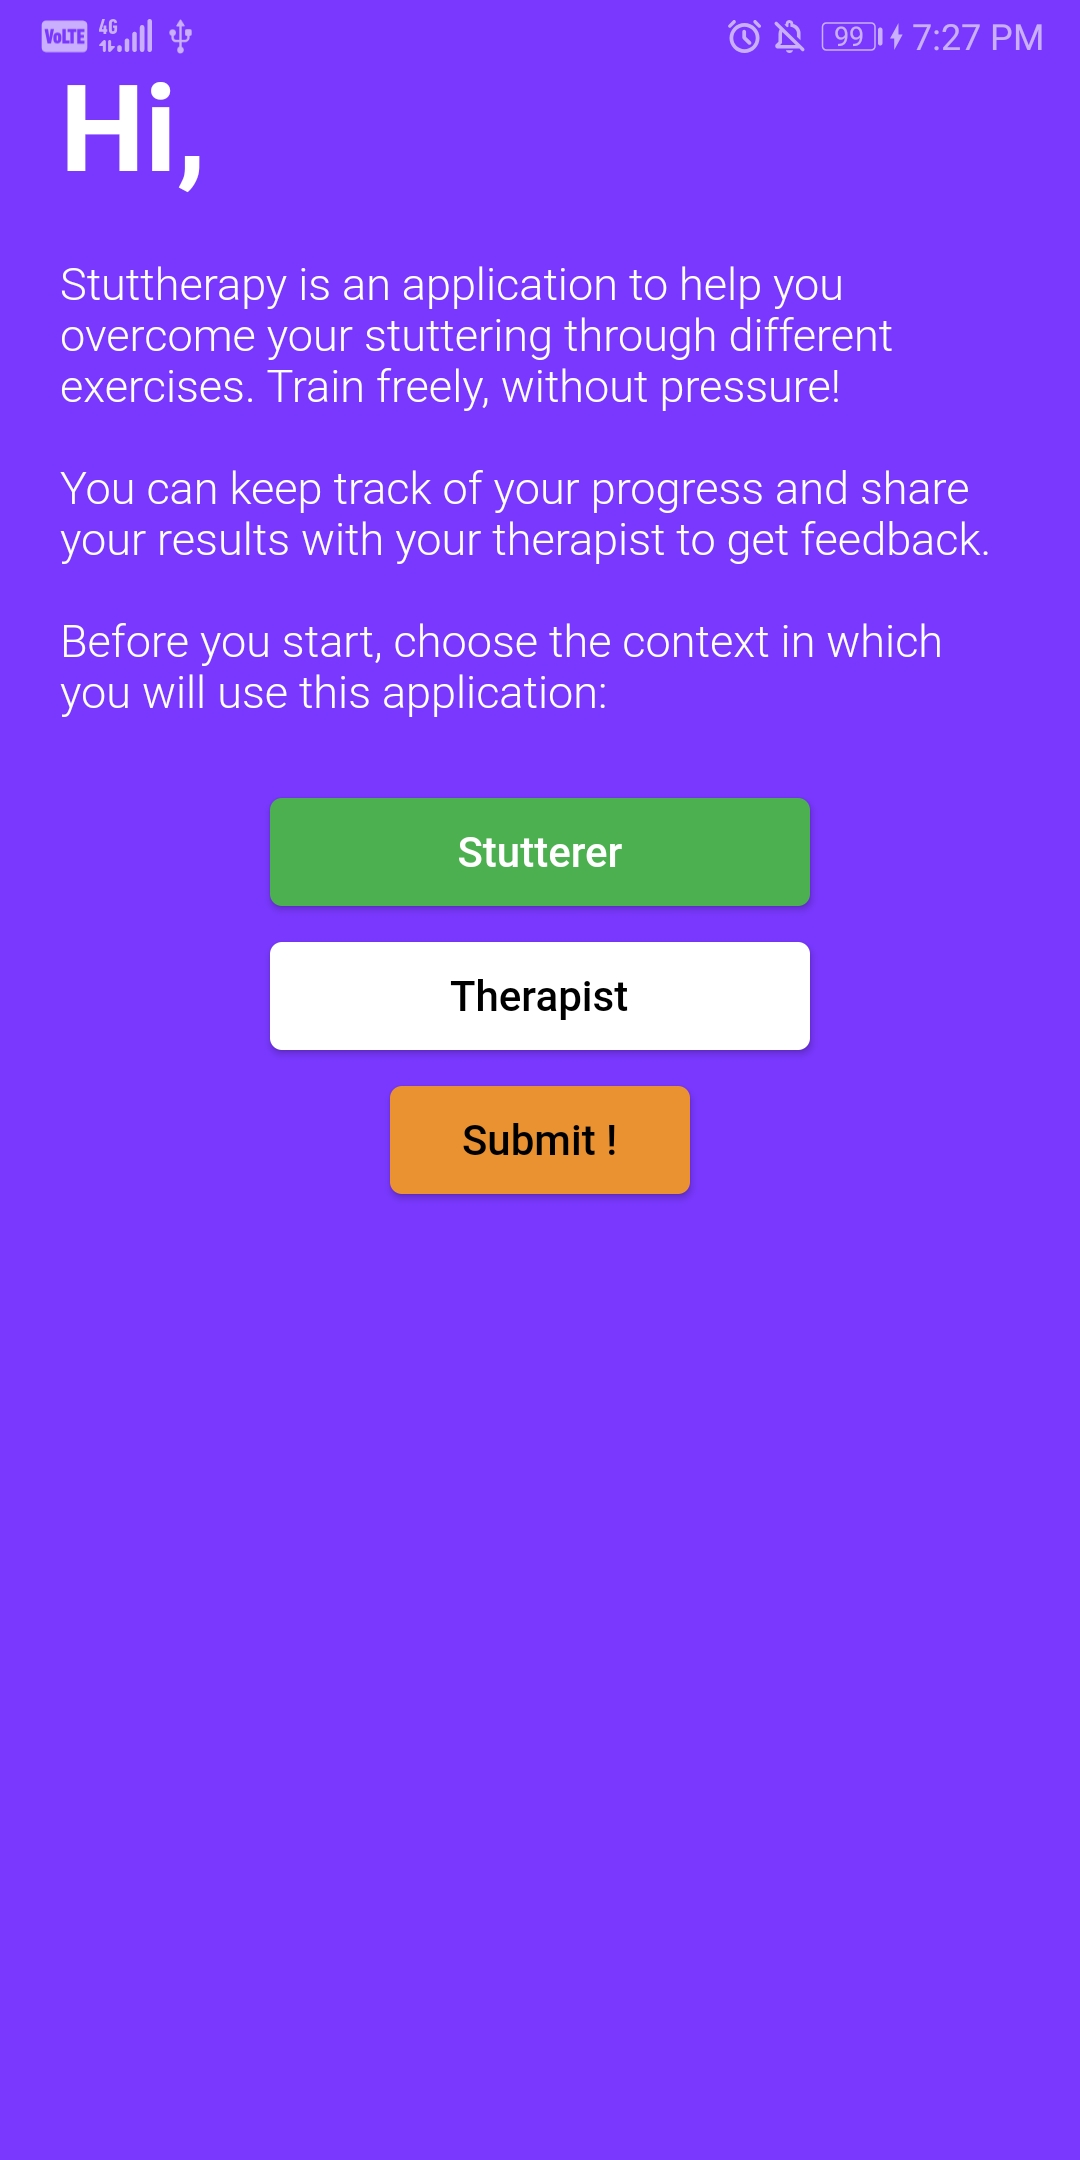
\includegraphics[width=.75\linewidth]{content/imgs/screen1.jpg}
    \caption{Page at first start}
  \end{subfigure}%
  \begin{subfigure}{.25\textwidth}
    \centering
    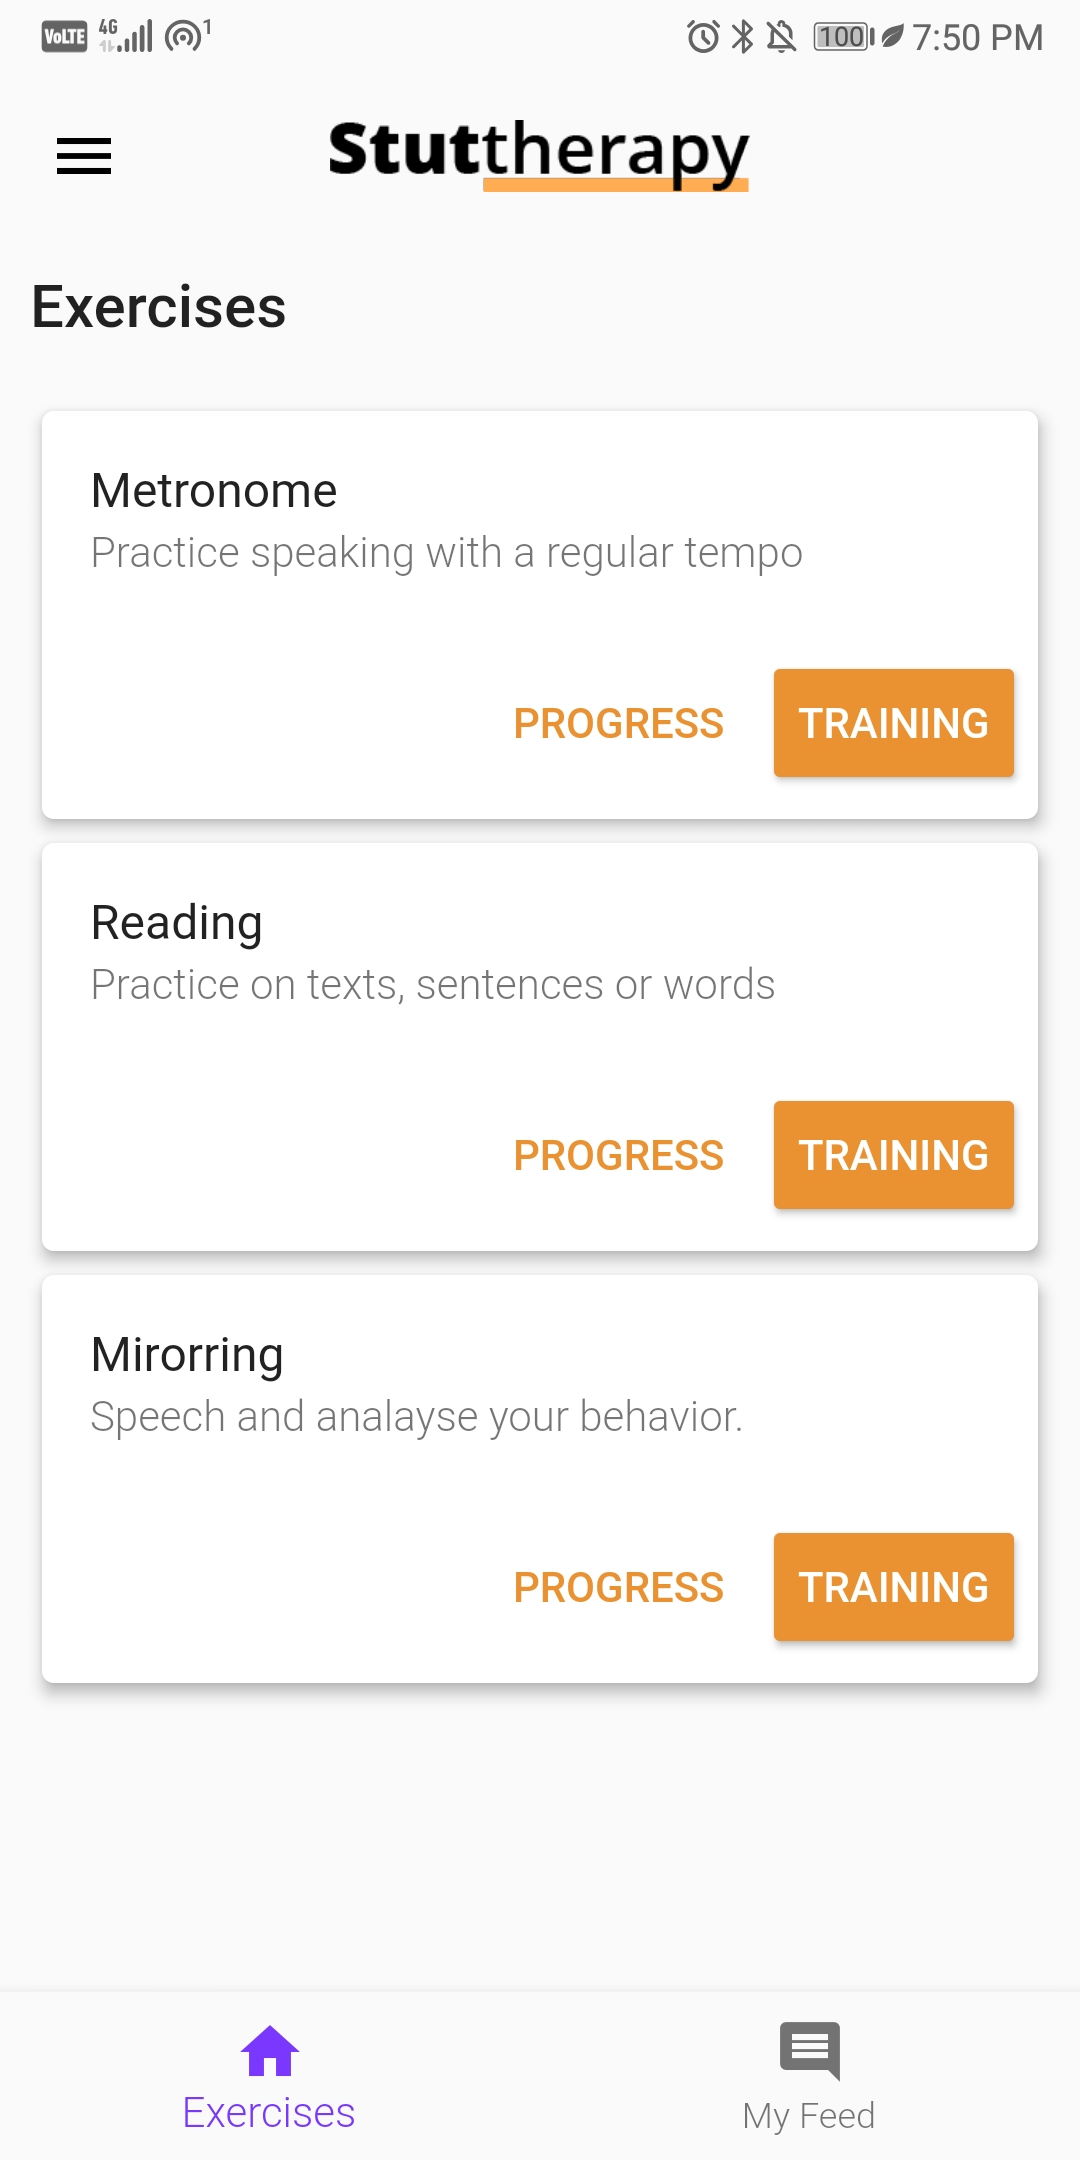
\includegraphics[width=.75\linewidth]{content/imgs/screen2.jpg}
    \caption{List of available exercises}
  \end{subfigure}%
  \begin{subfigure}{.25\textwidth}
    \centering
    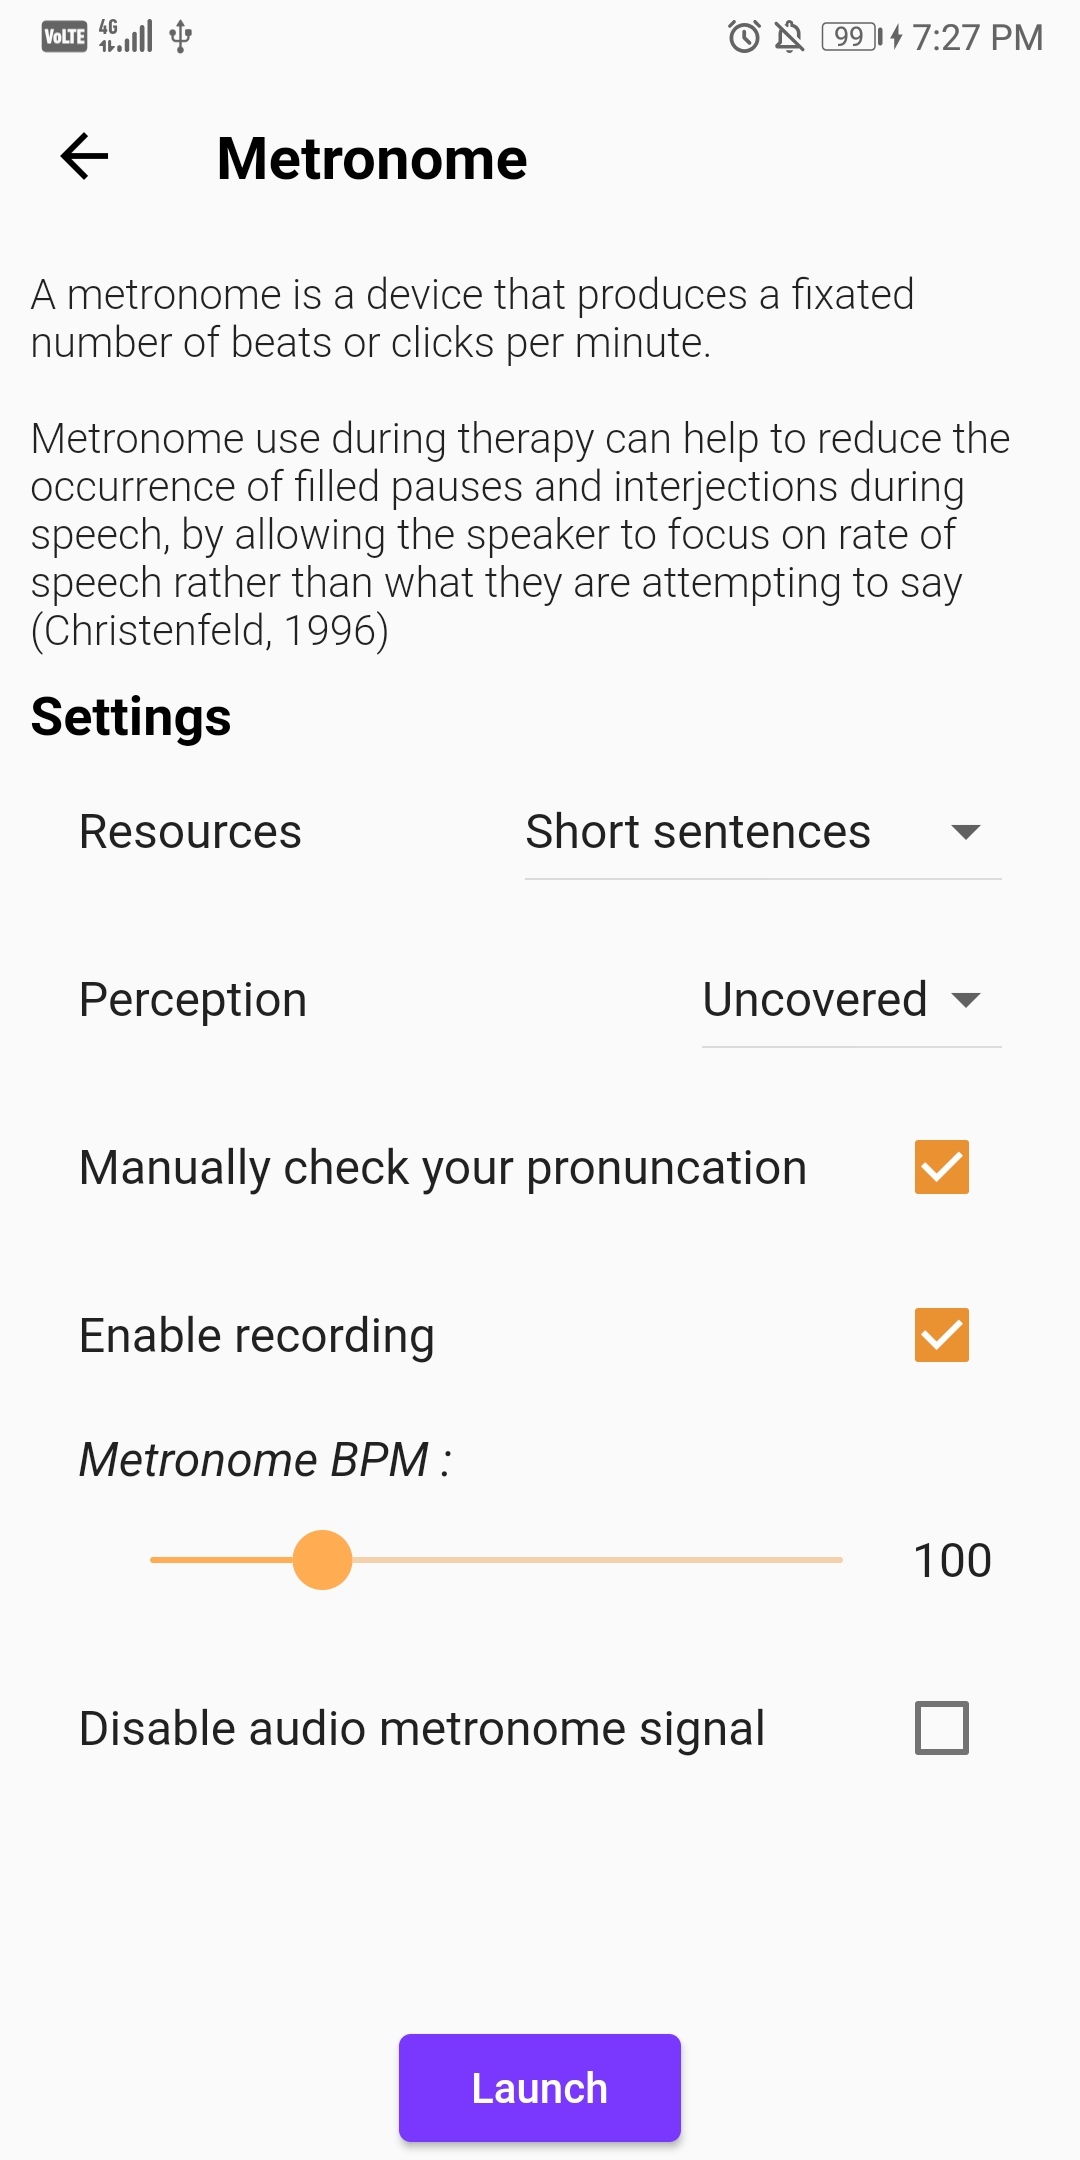
\includegraphics[width=.75\linewidth]{content/imgs/screen3.jpg}
    \caption{Exercise homepage \textit{metronome}}
  \end{subfigure}%
  \begin{subfigure}{.25\textwidth}
    \centering
    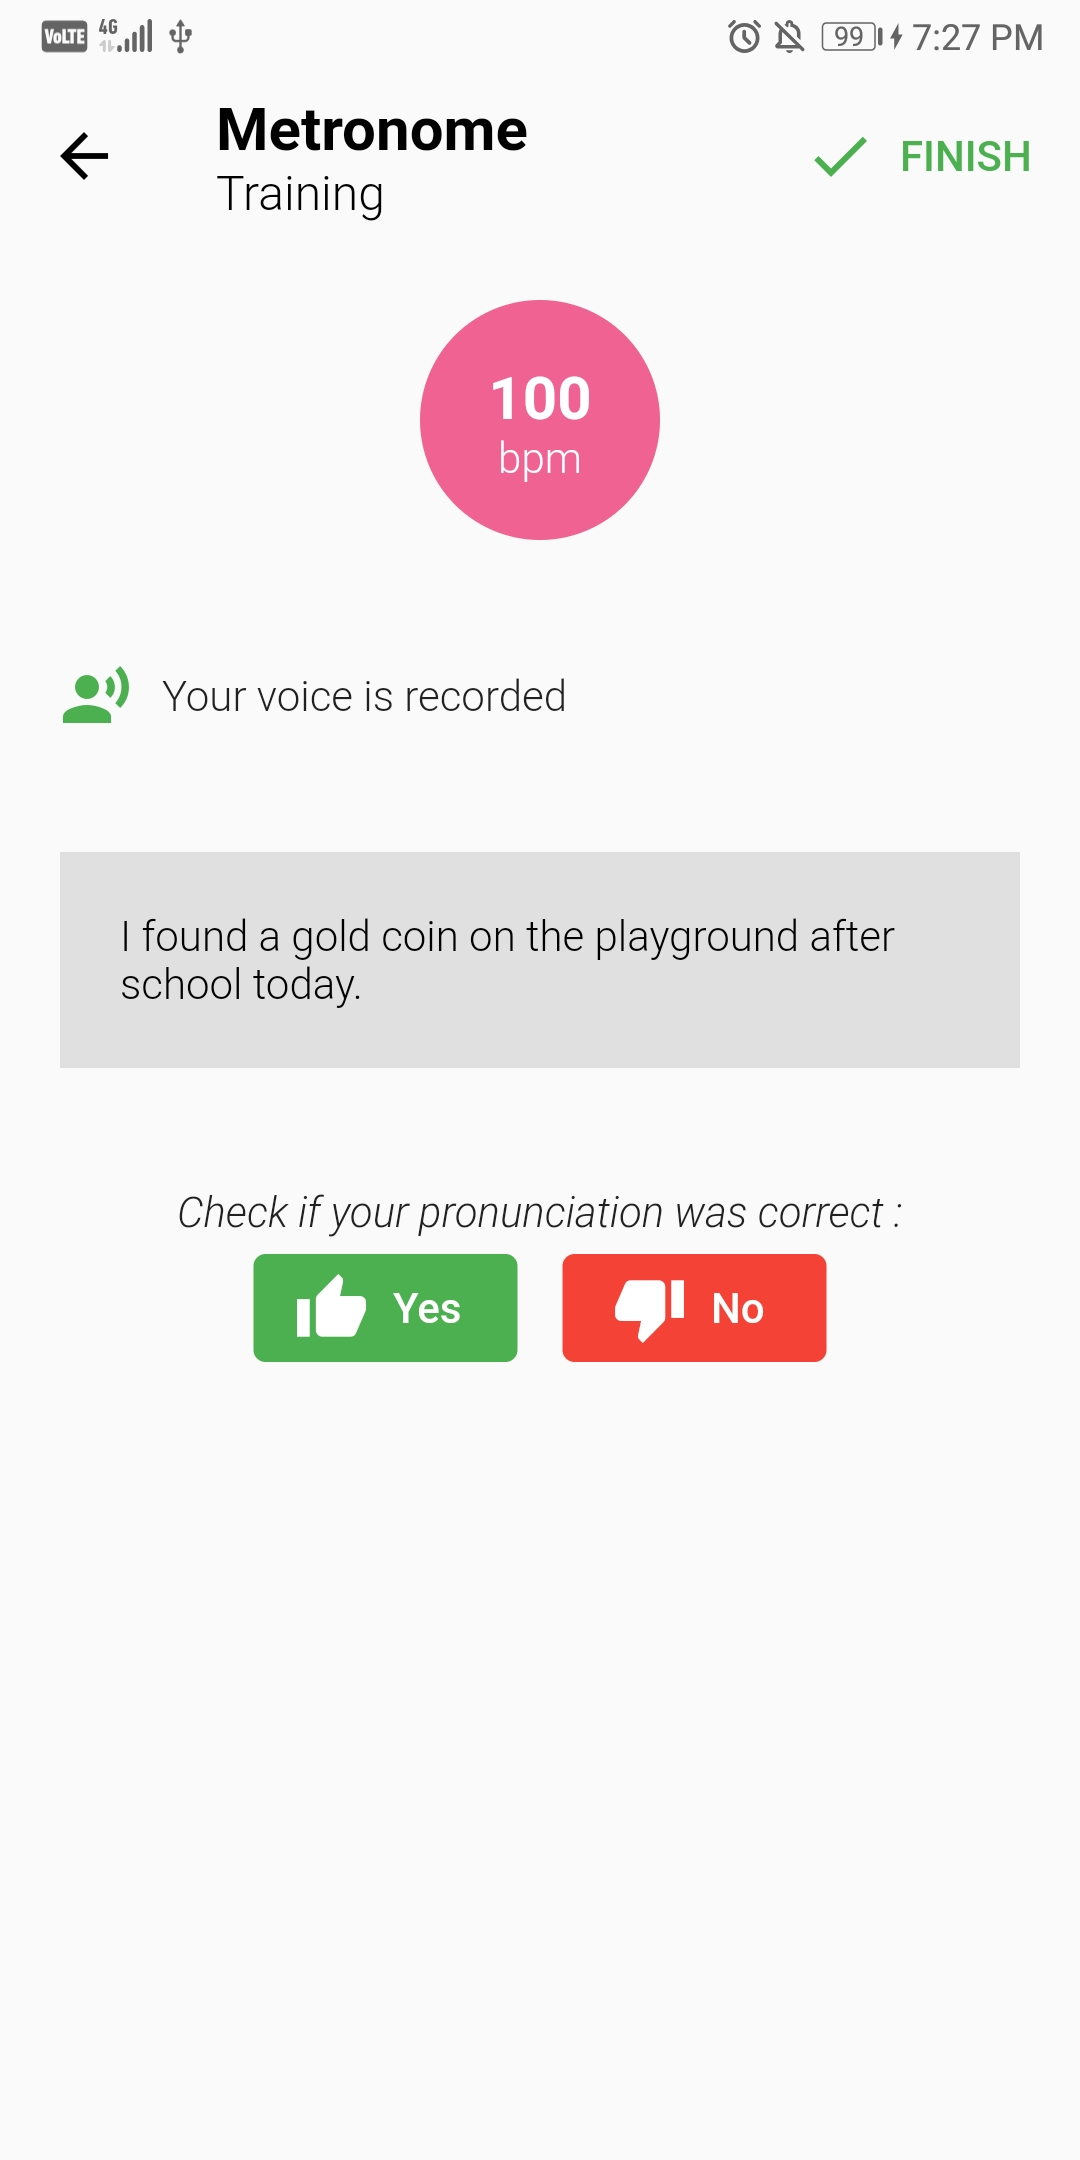
\includegraphics[width=.75\linewidth]{content/imgs/screen4.jpg}
    \caption{Exercise training on the exercise \textit{metronome}}
  \end{subfigure}
\end{figure}


\begin{figure}[h]
  \begin{subfigure}{.25\textwidth}
    \centering
    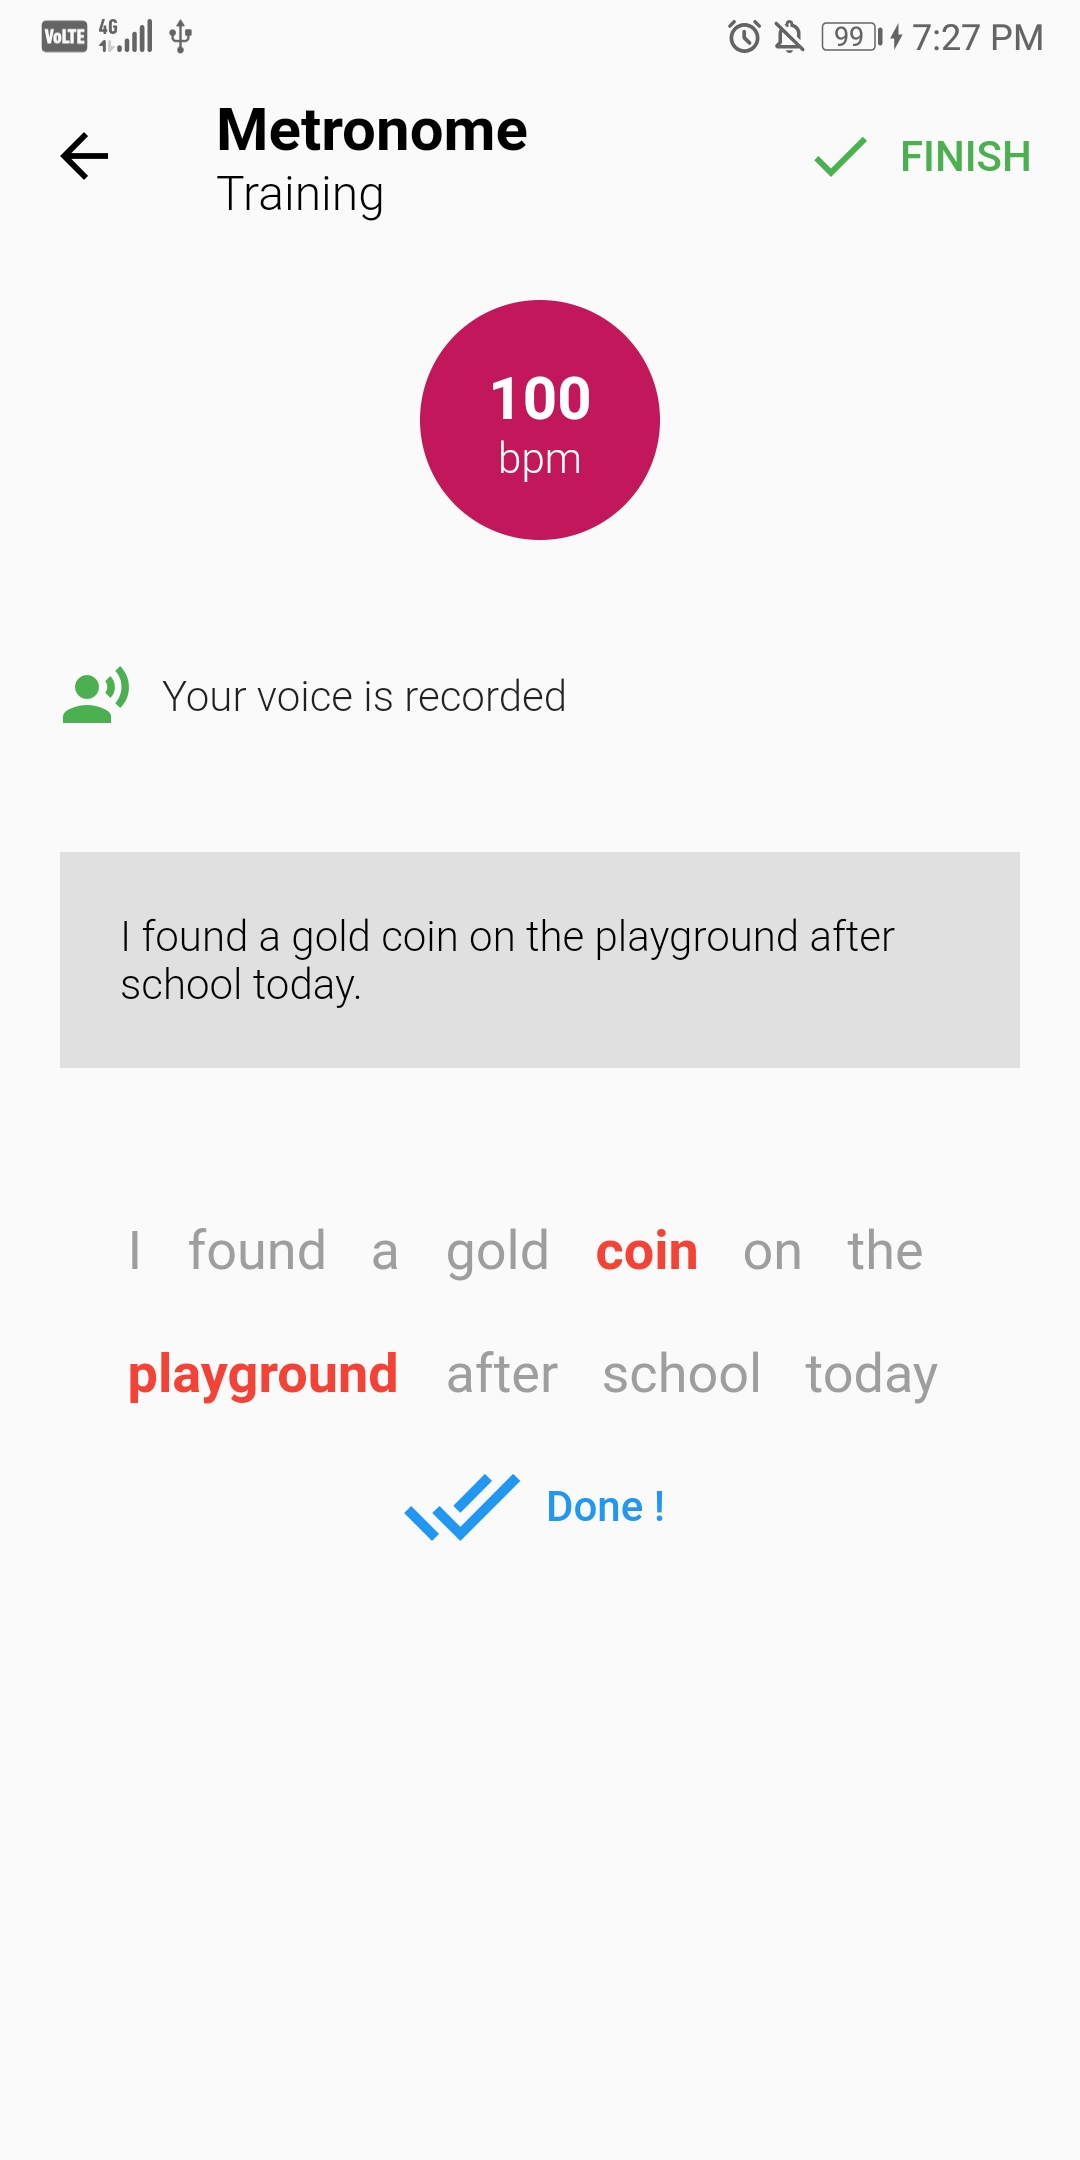
\includegraphics[width=.75\linewidth]{content/imgs/screen5.jpg}
    \caption{Selection of mispronounced words}
  \end{subfigure}%
  \begin{subfigure}{.25\textwidth}
    \centering
    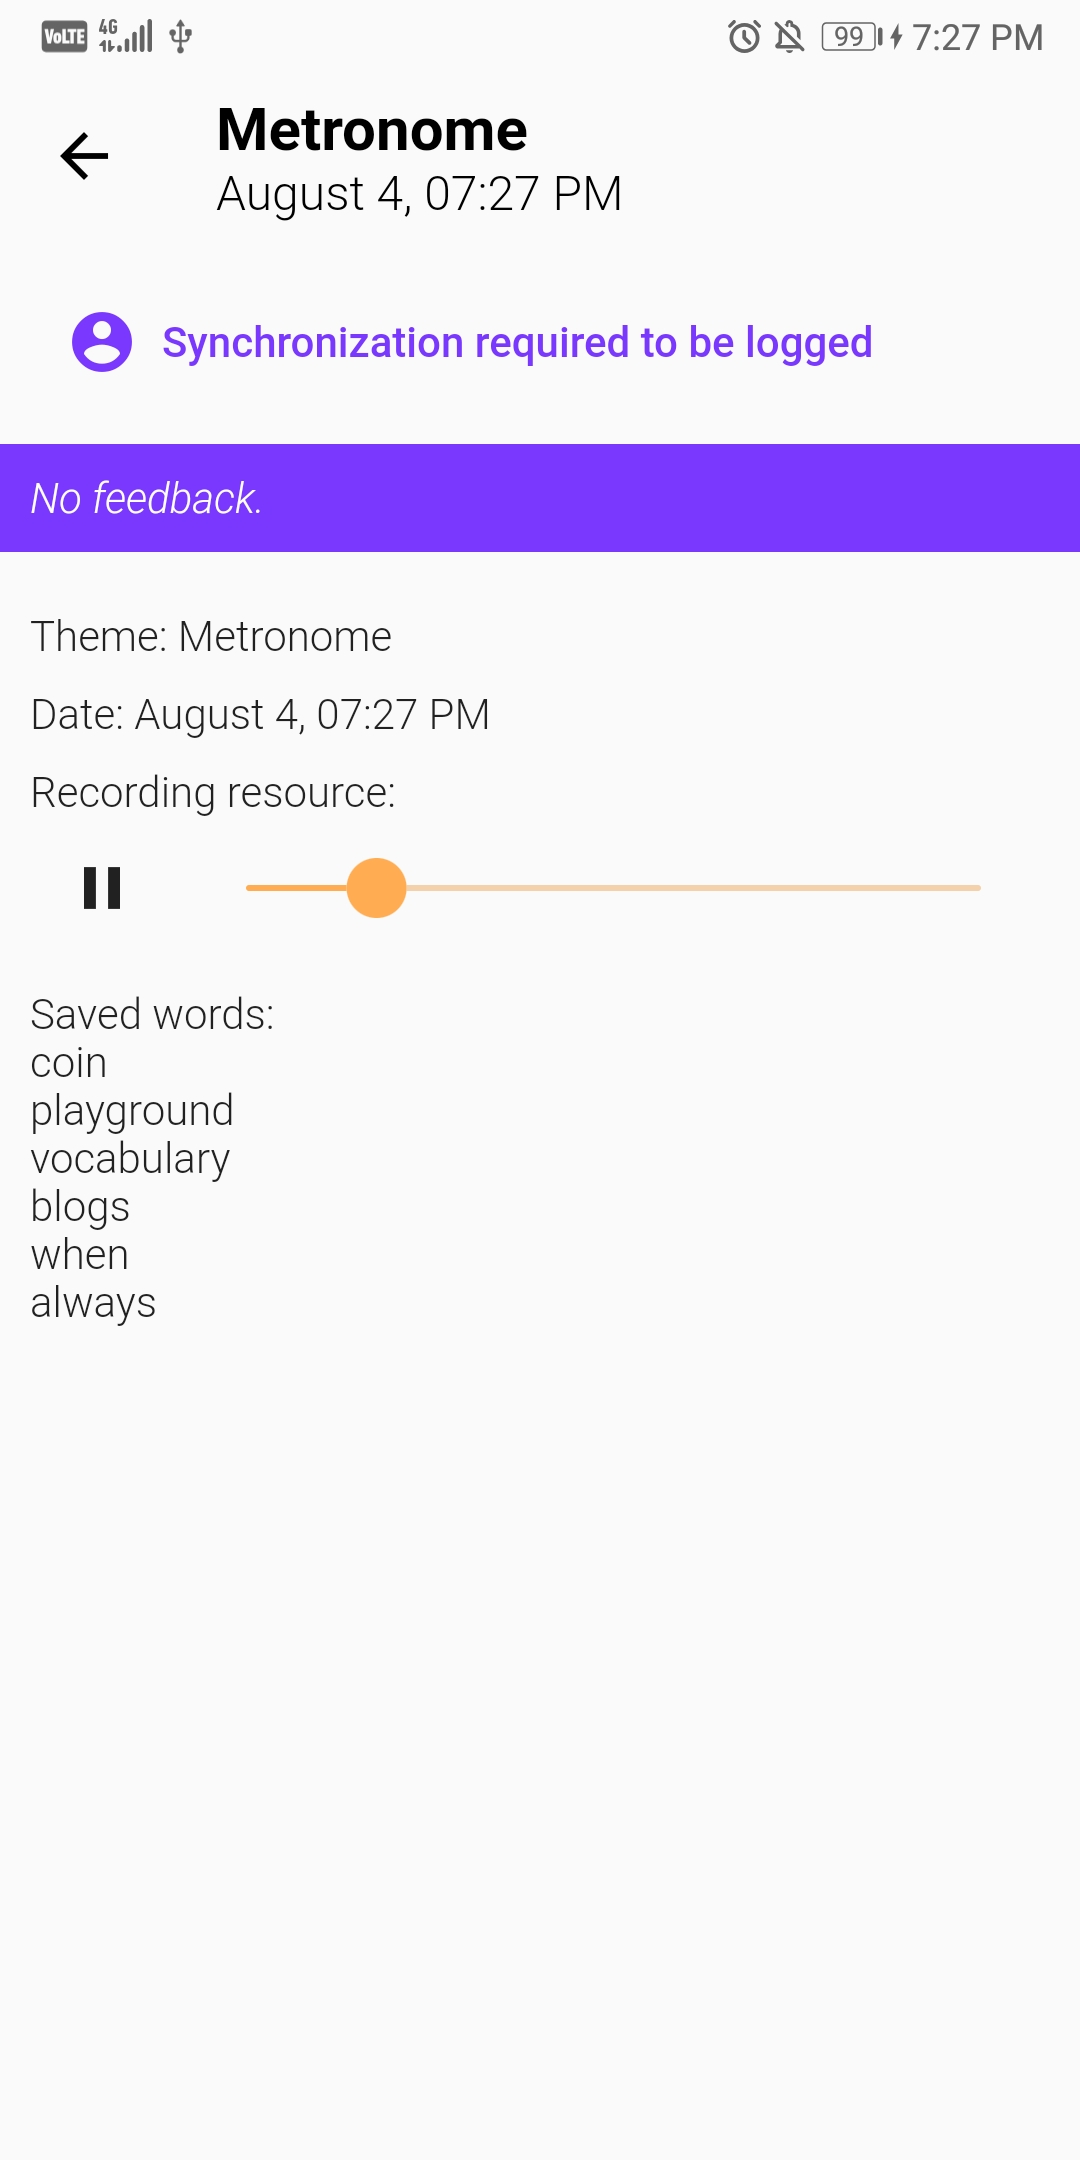
\includegraphics[width=.75\linewidth]{content/imgs/screen6.jpg}
    \caption{End of the exercise, summary}
  \end{subfigure}%
  \begin{subfigure}{.25\textwidth}
    \centering
    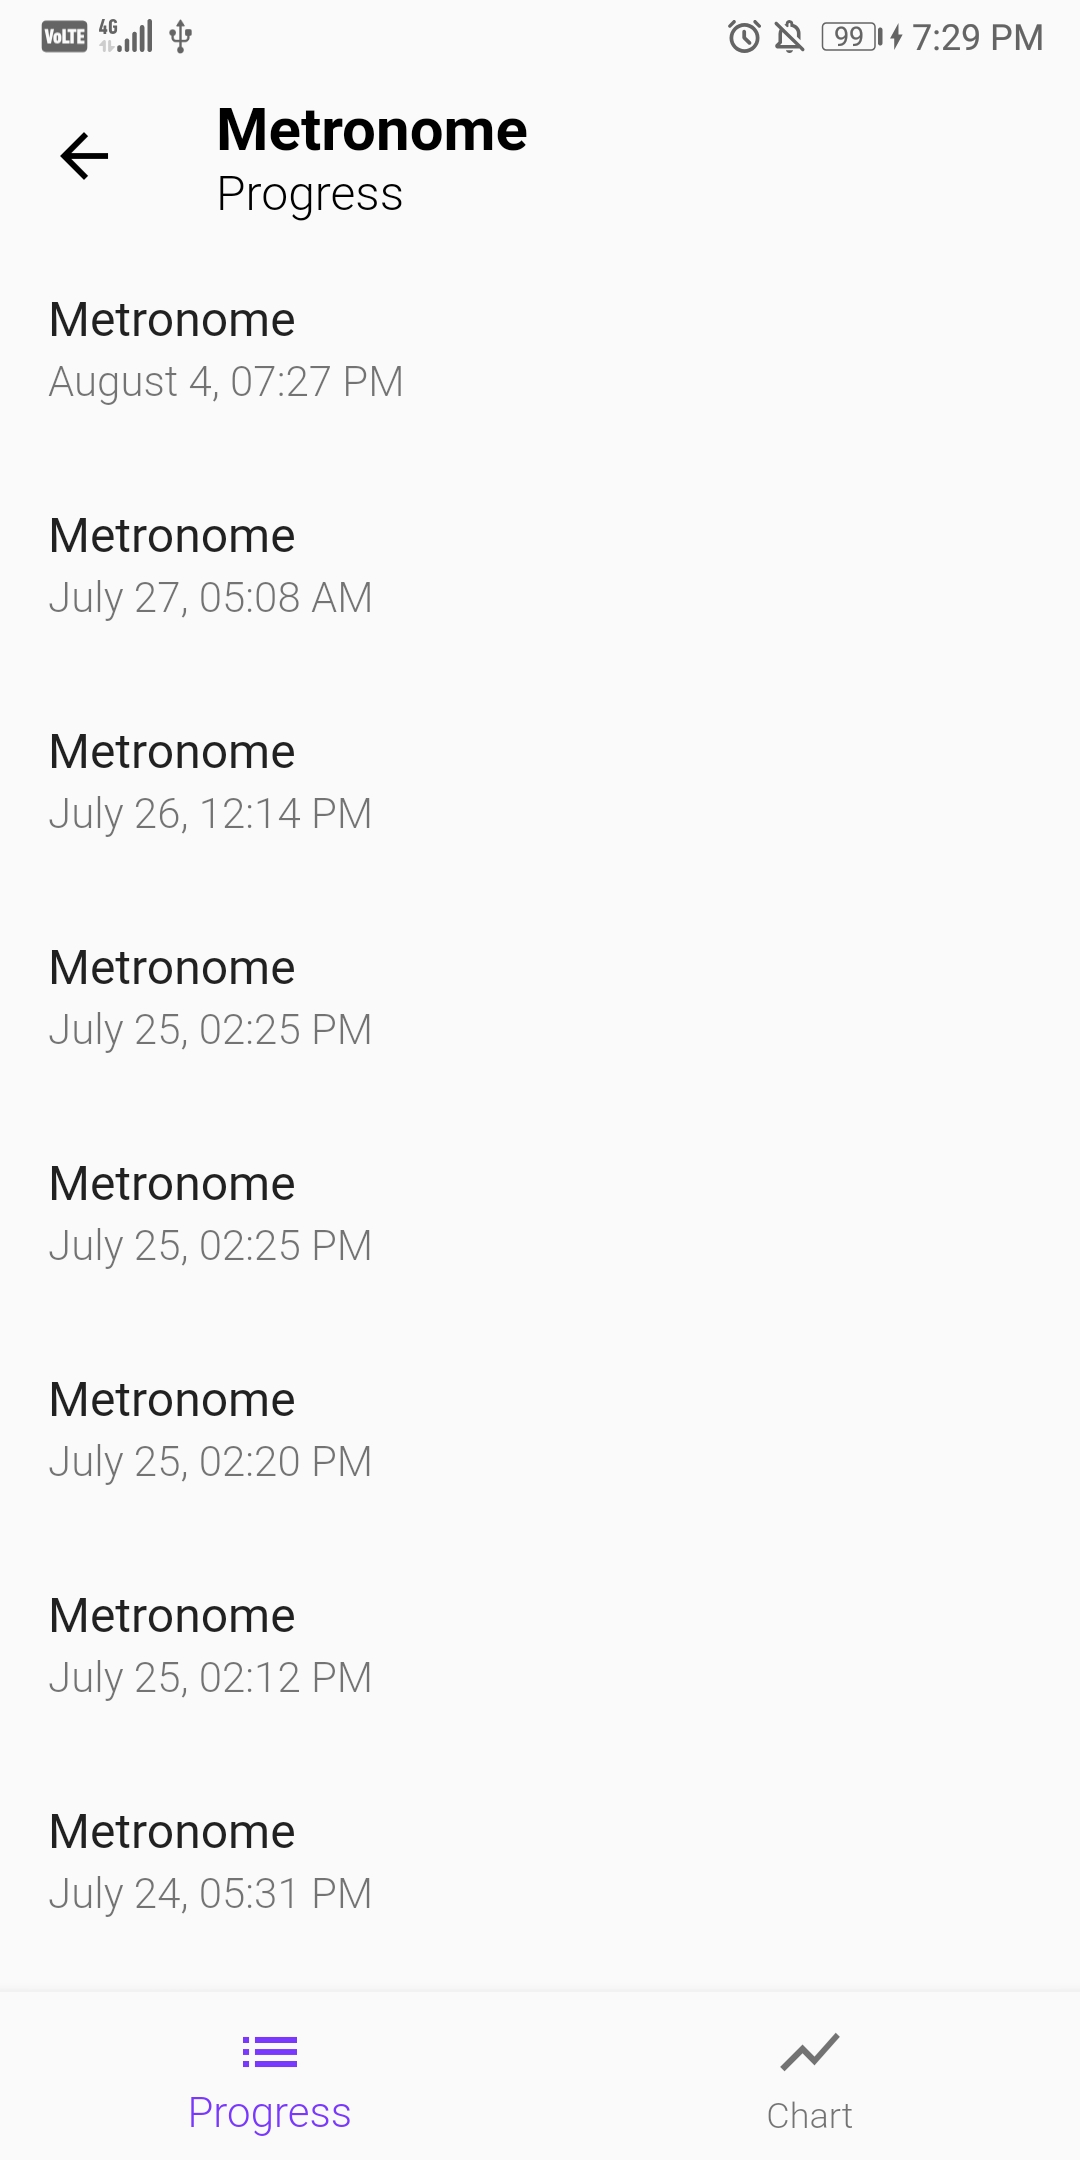
\includegraphics[width=.75\linewidth]{content/imgs/screen7.jpg}
    \caption{List of all the exercises performed with the exercise \textit{metronome}}
  \end{subfigure}%
  \begin{subfigure}{.25\textwidth}
    \centering
    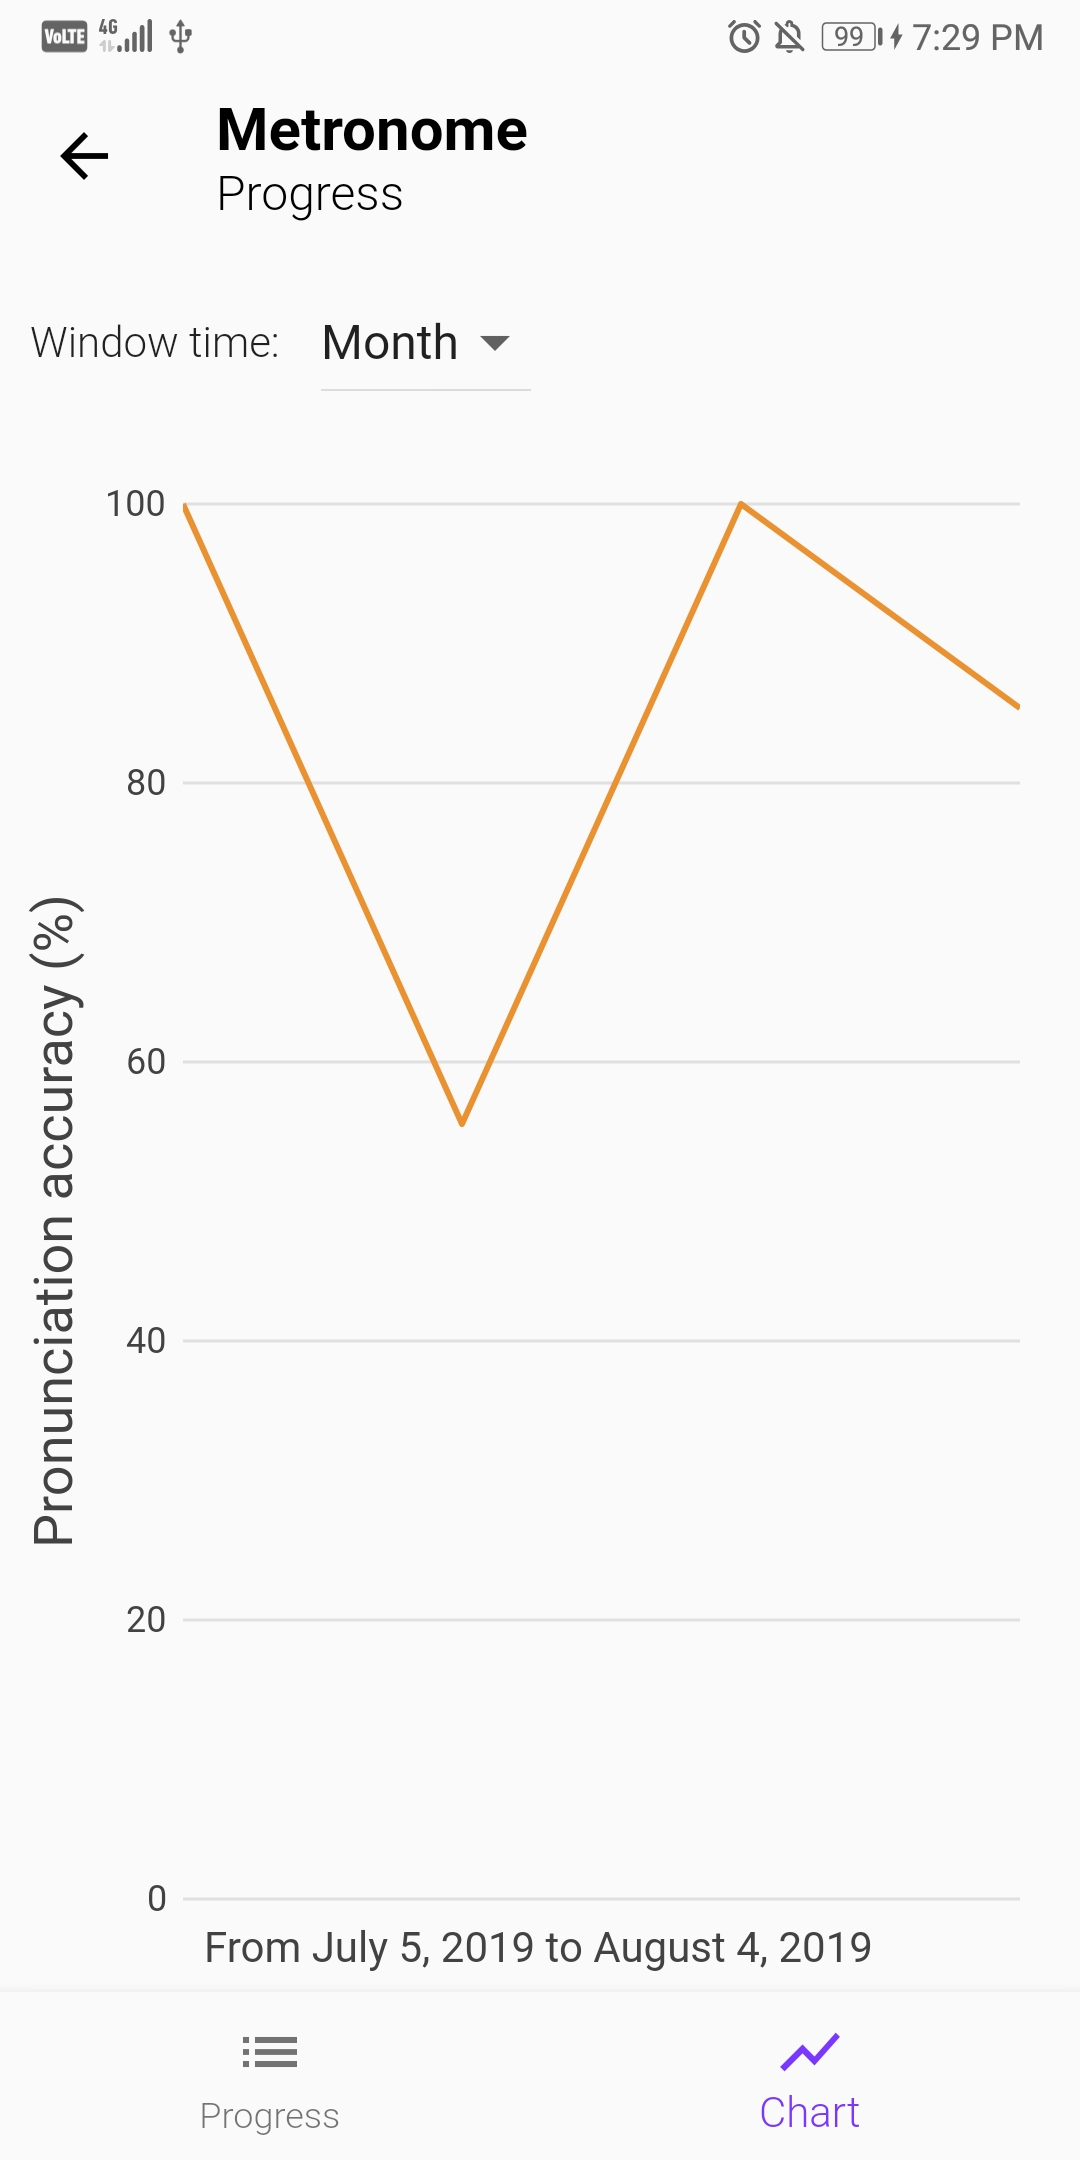
\includegraphics[width=.75\linewidth]{content/imgs/screen8.jpg}
    \caption{Progress line chart over the year \textit{metronome}}
  \end{subfigure}
\end{figure}


\begin{figure}[h]
  \begin{subfigure}{.25\textwidth}
    \centering
    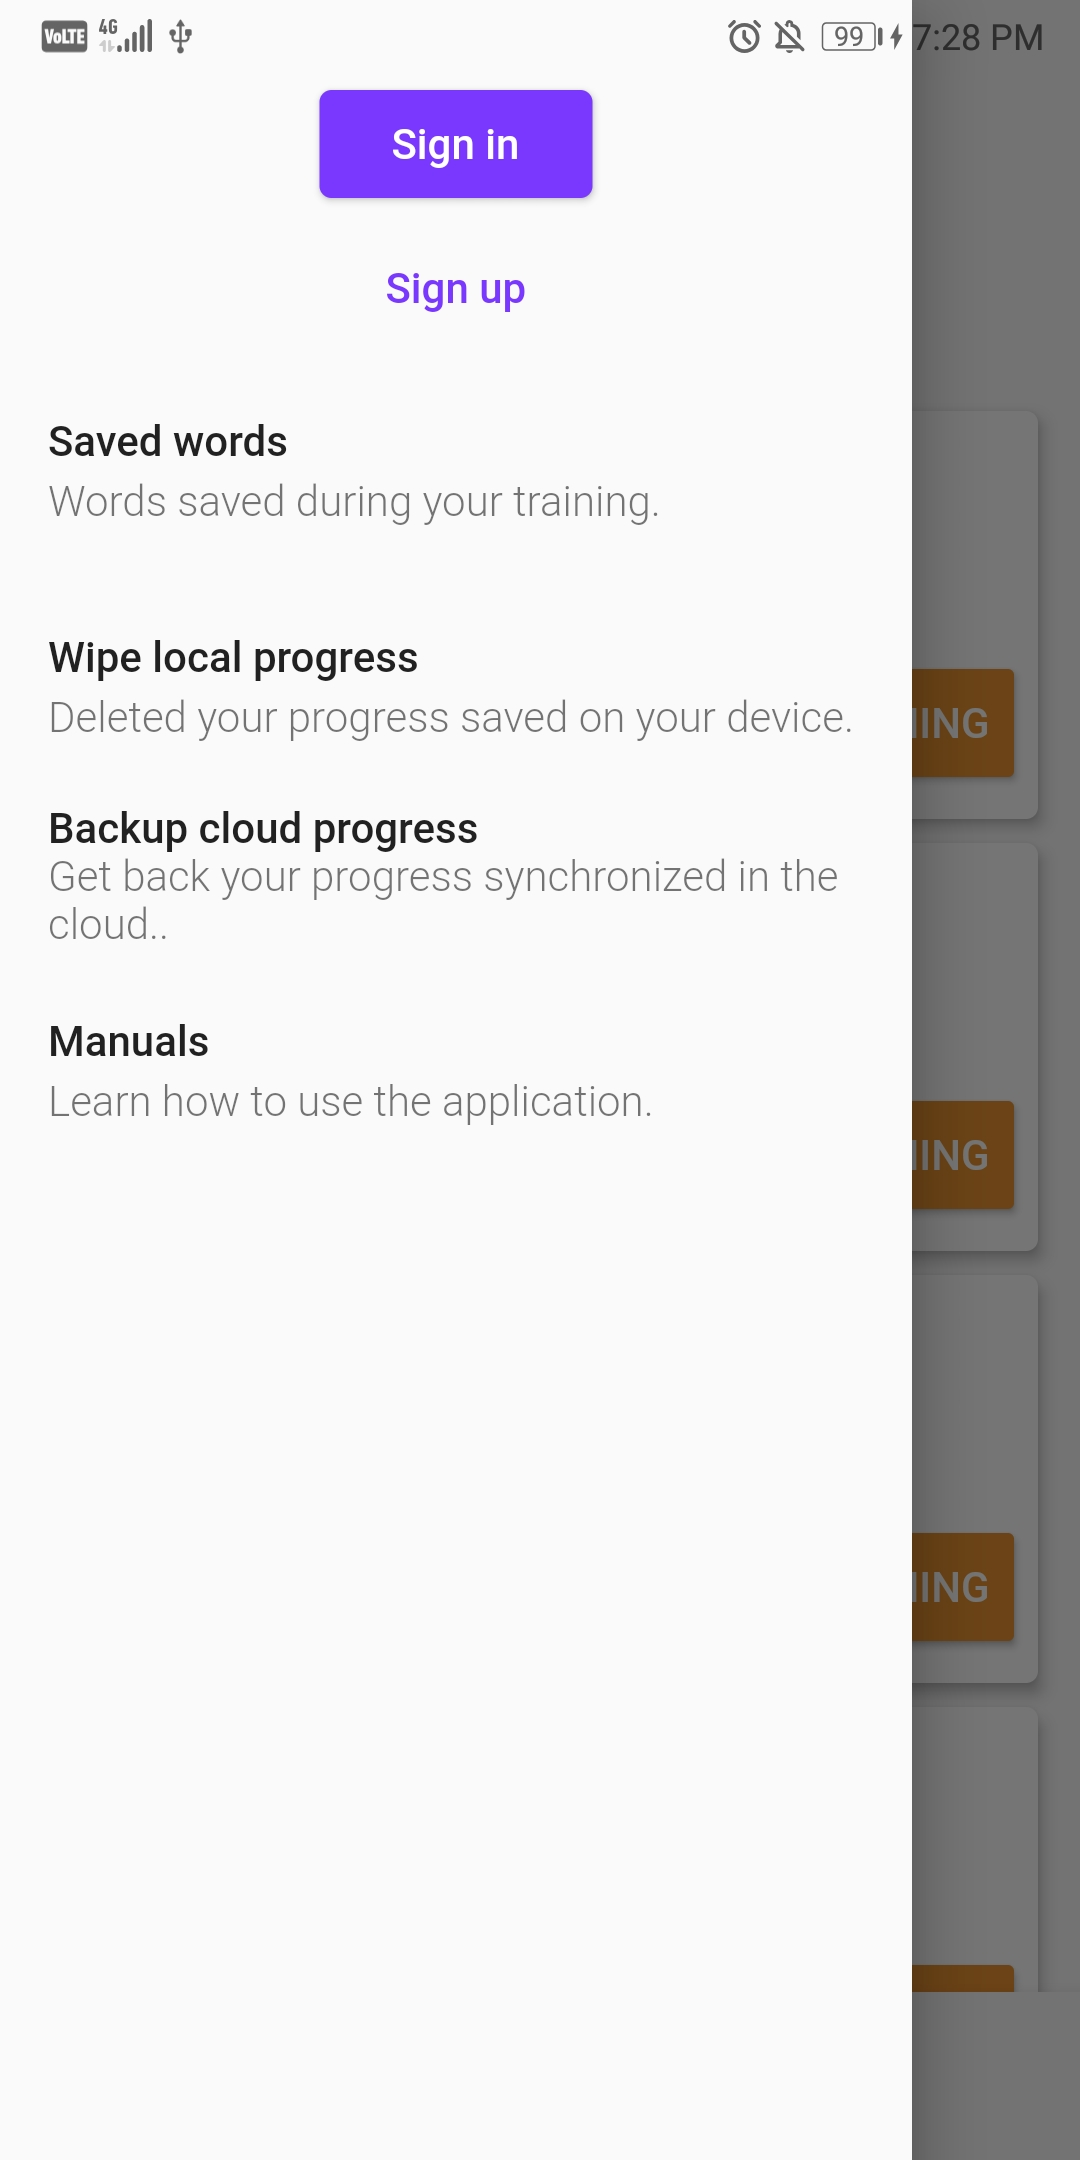
\includegraphics[width=.75\linewidth]{content/imgs/screen9.jpg}
    \caption{Application menu}
  \end{subfigure}%
  \begin{subfigure}{.25\textwidth}
    \centering
    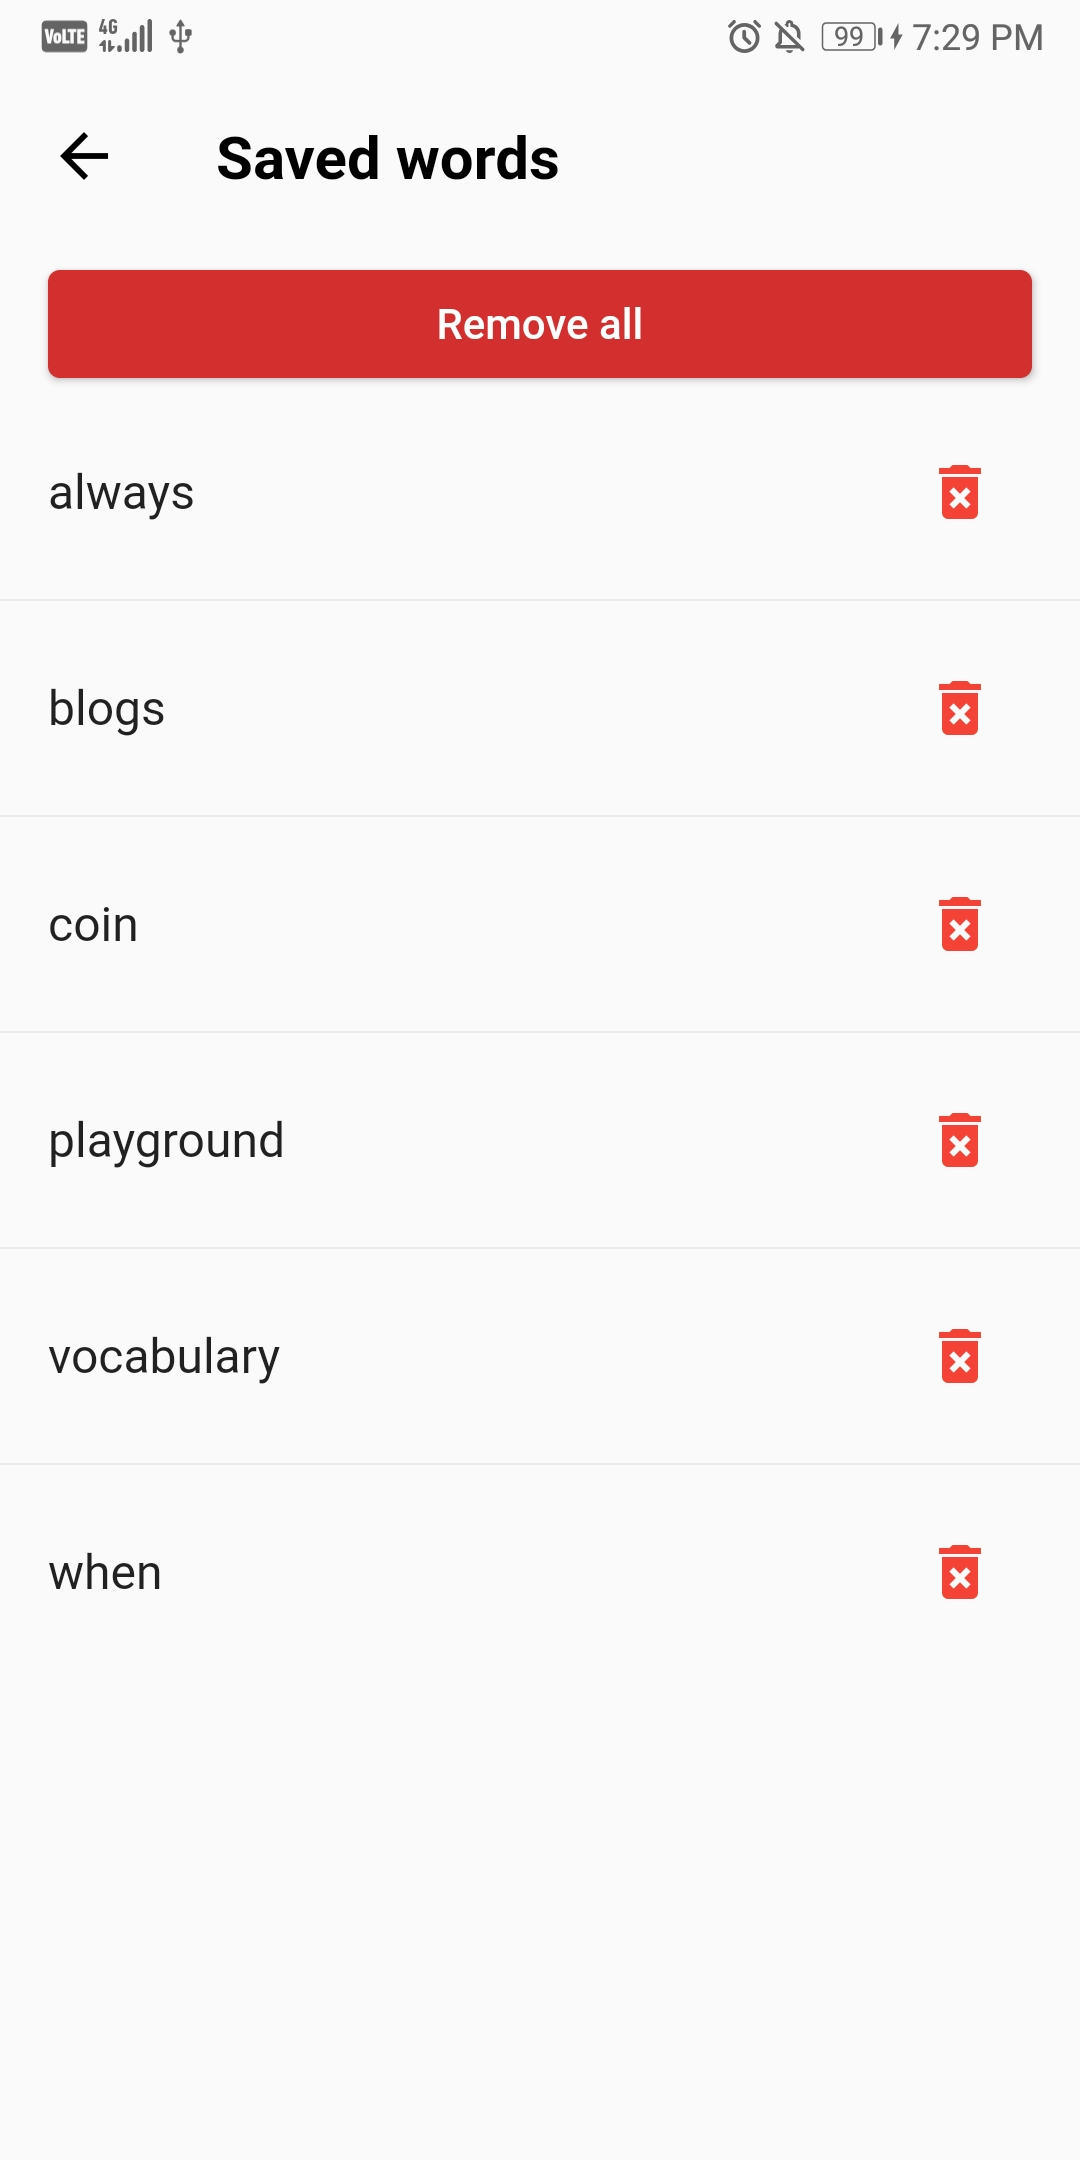
\includegraphics[width=.75\linewidth]{content/imgs/screen10.jpg}
    \caption{Words mispronounced during the exercises}
  \end{subfigure}%
  \begin{subfigure}{.25\textwidth}
    \centering
    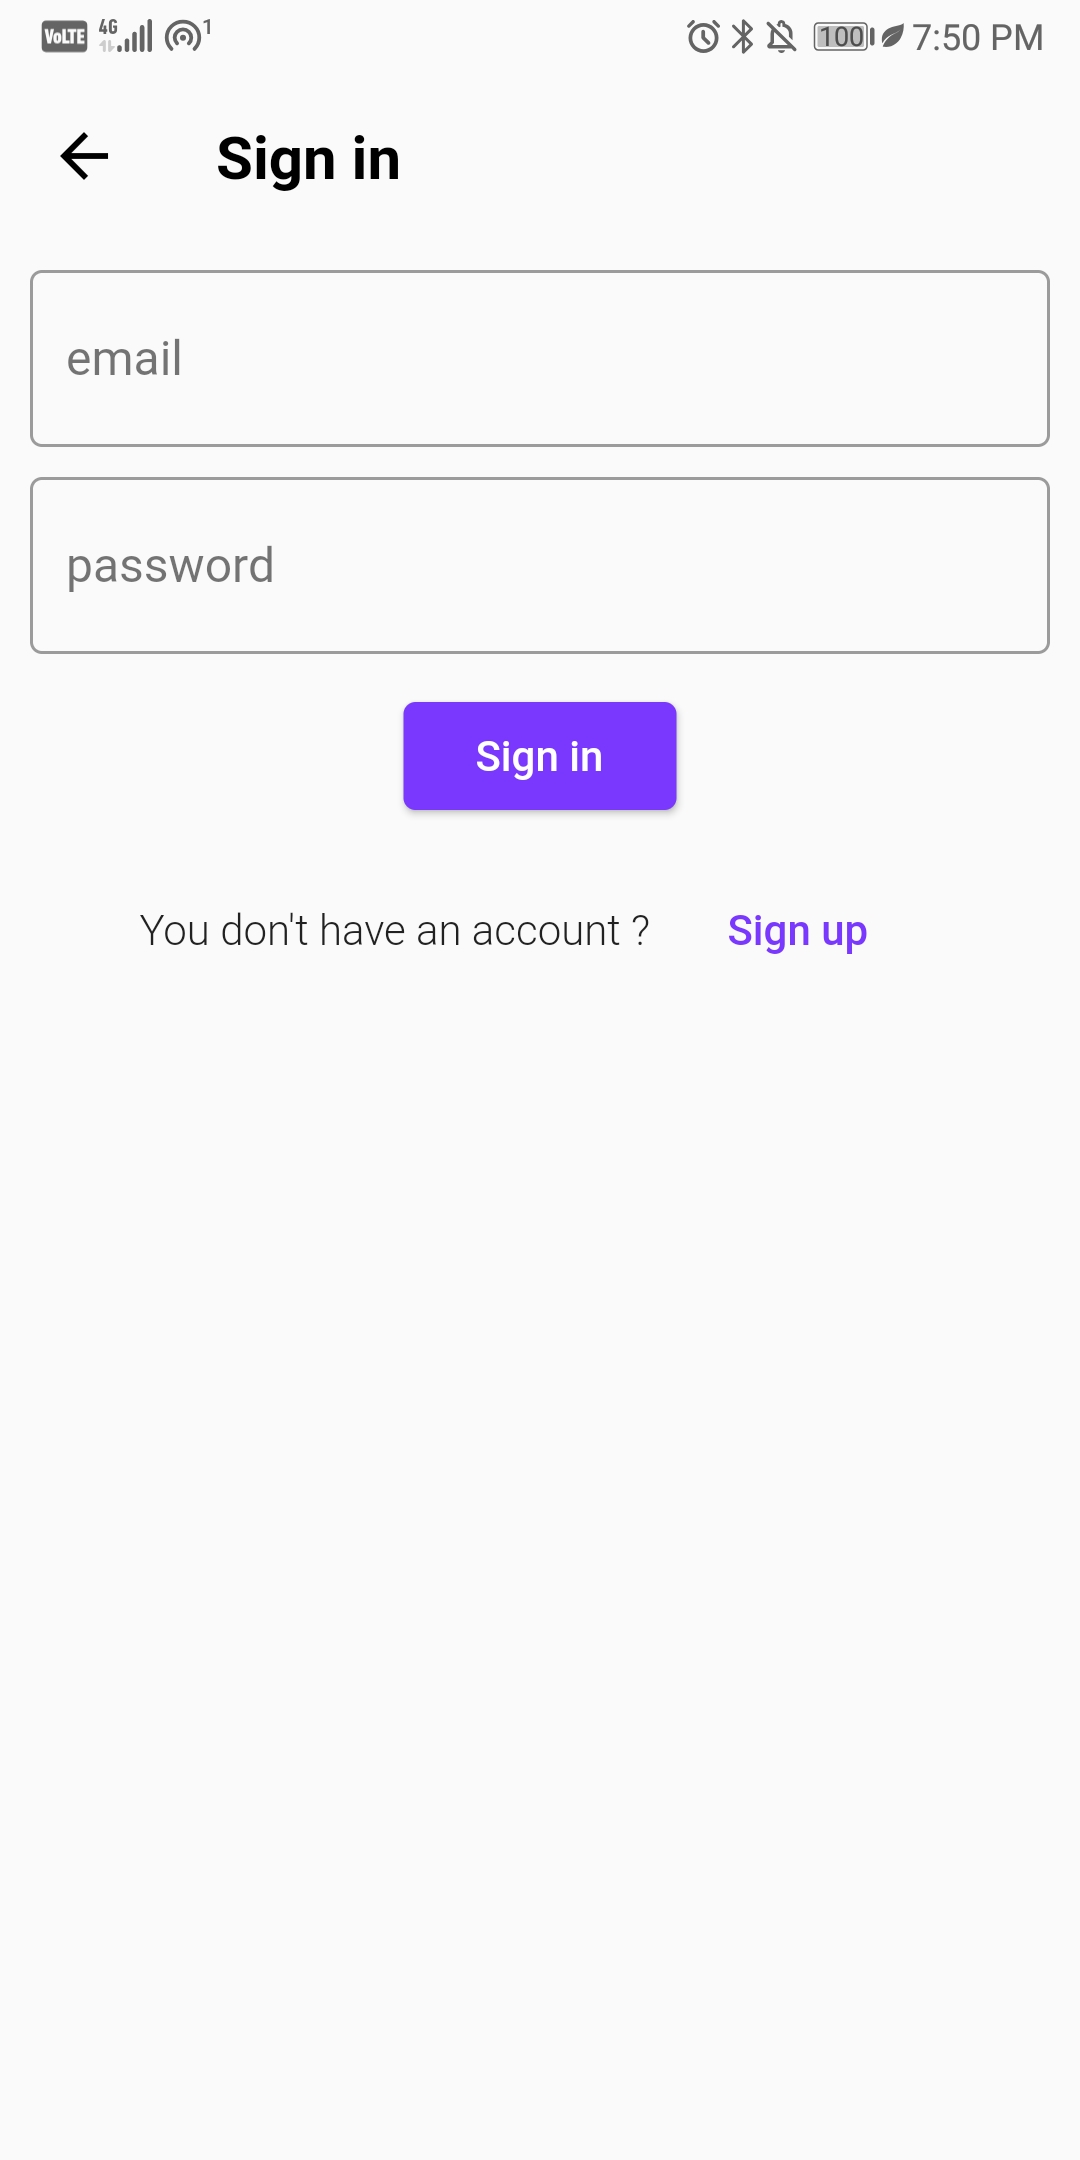
\includegraphics[width=.75\linewidth]{content/imgs/screen11.jpg}
    \caption{Login Form}
  \end{subfigure}%
  \begin{subfigure}{.25\textwidth}
    \centering
    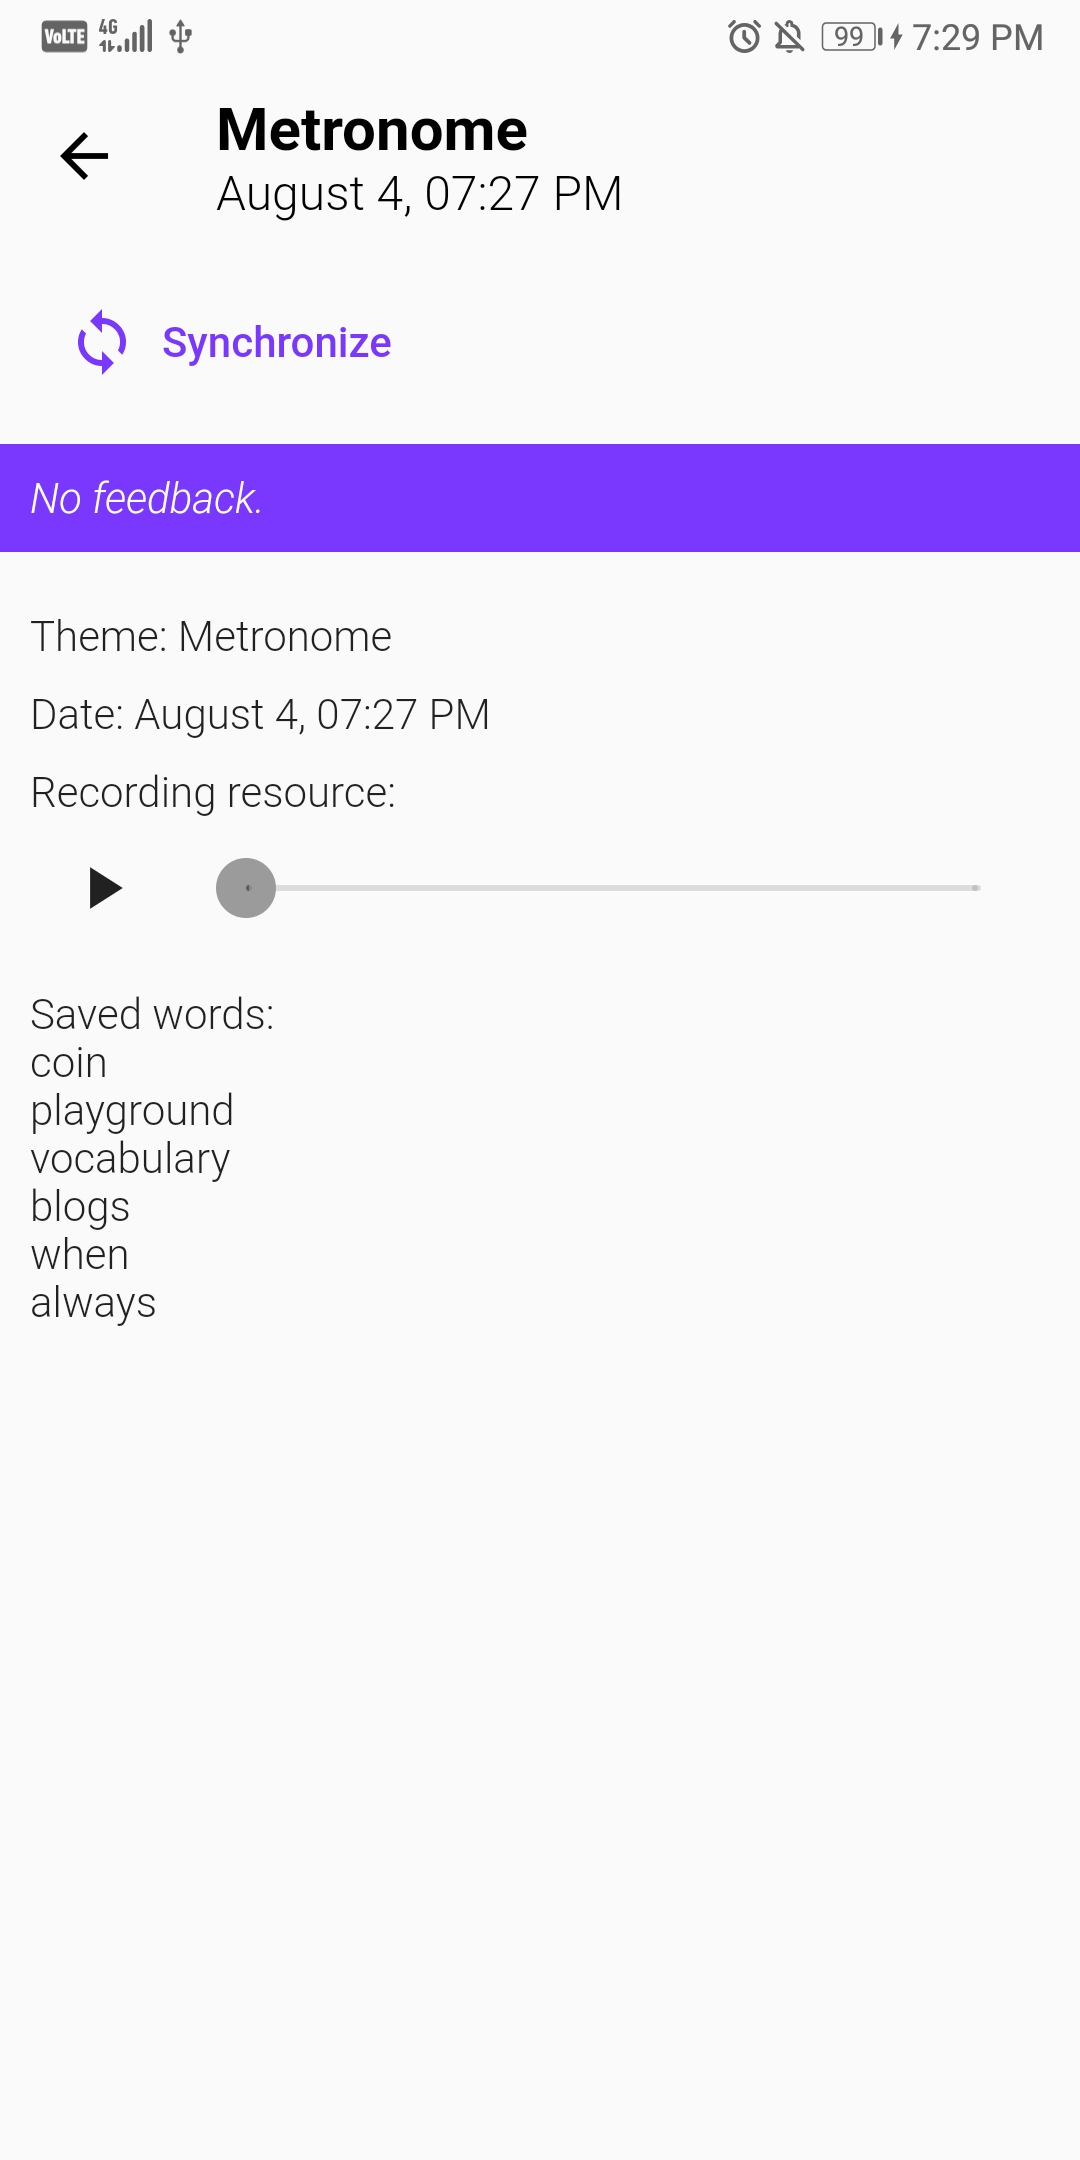
\includegraphics[width=.75\linewidth]{content/imgs/screen12.jpg}
    \caption{History of an exercise with possible synchronization}
  \end{subfigure}
\end{figure}


\begin{figure}[h]
  \begin{subfigure}{.25\textwidth}
    \centering
    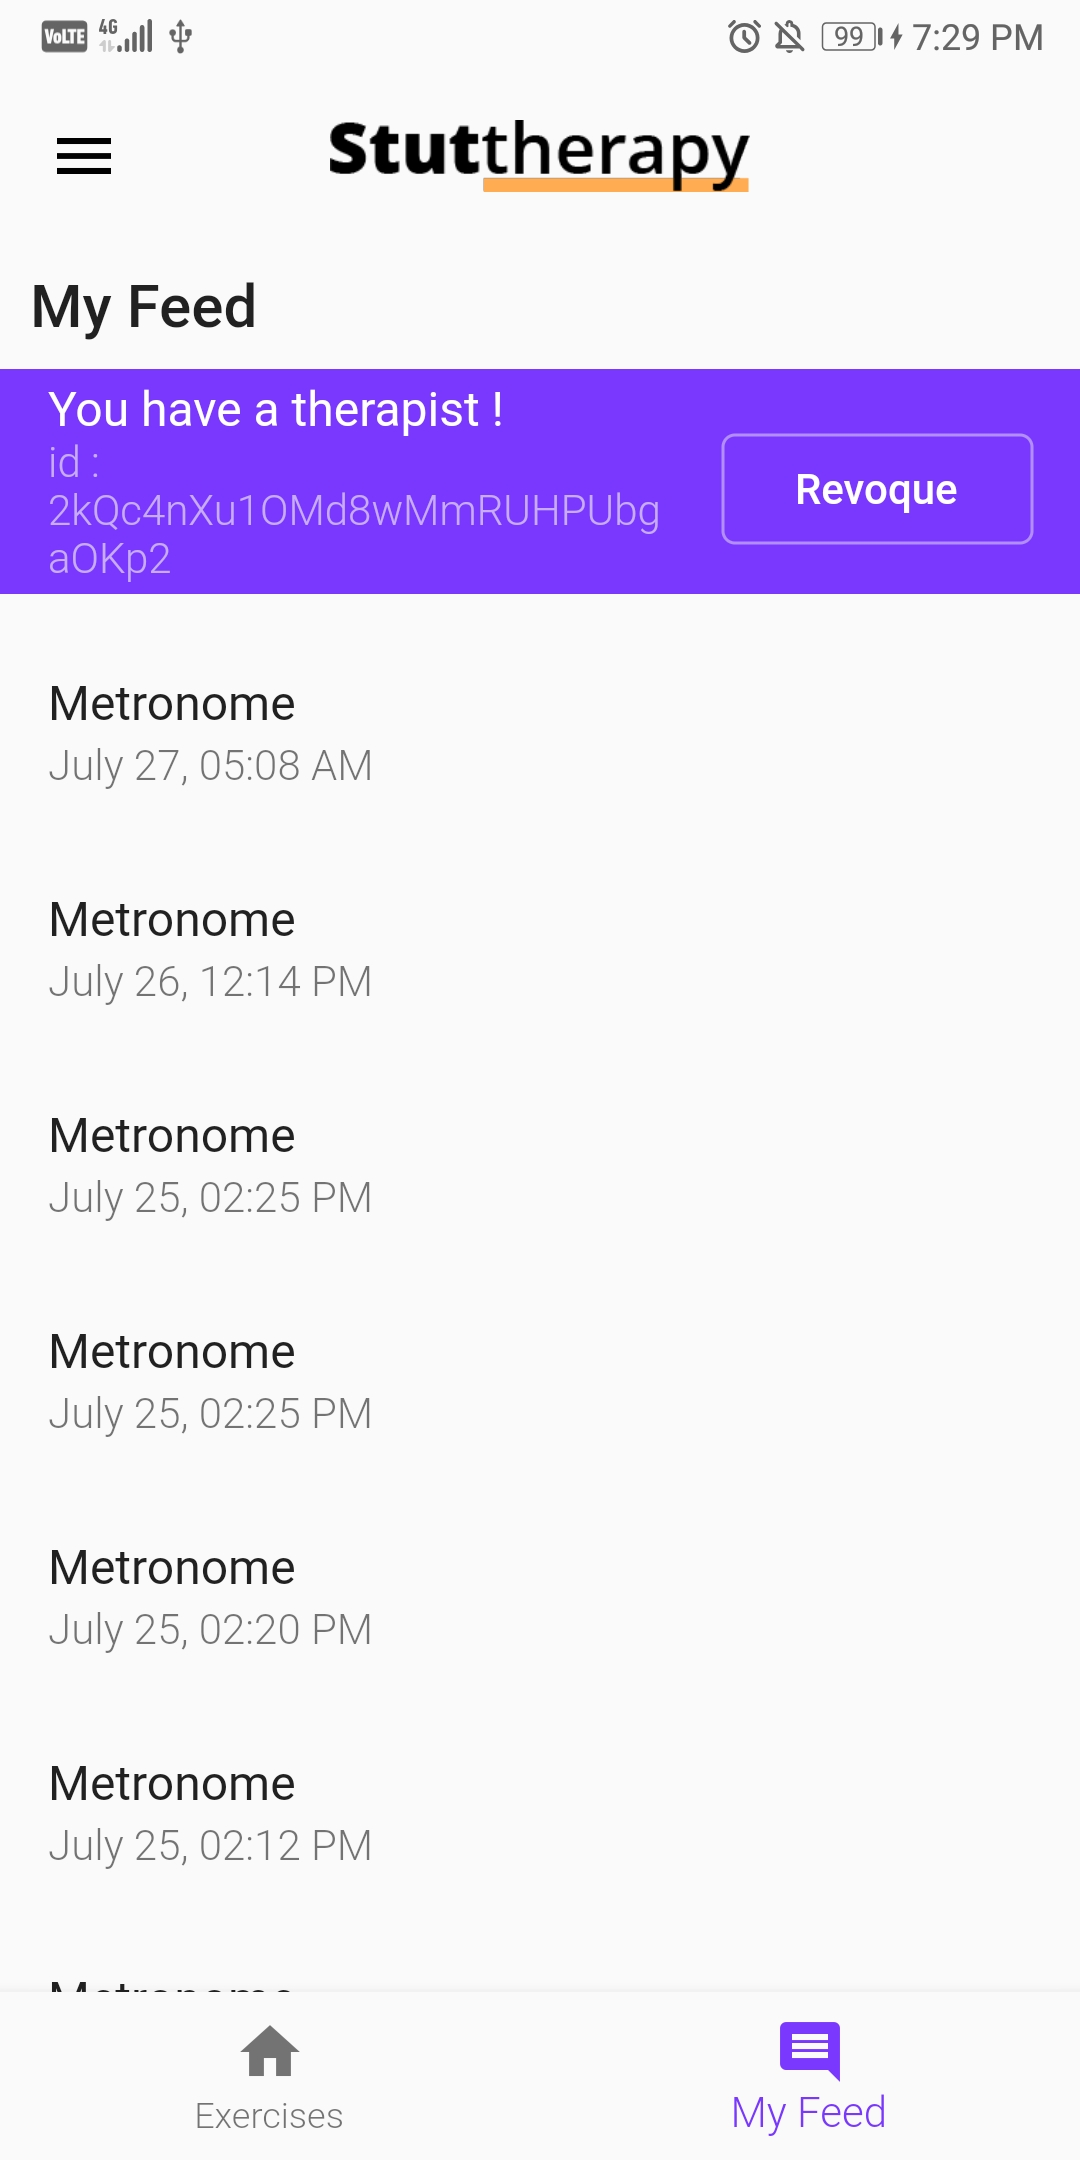
\includegraphics[width=.75\linewidth]{content/imgs/screen13.jpg}
    \caption{Data synchronized with a speech-language pathologist}
  \end{subfigure}%
  \begin{subfigure}{.25\textwidth}
    \centering
    
\includegraphics[width=.75\linewidth]{content/imgs/screen14.jpg}
    \caption{Speech therapist Home Page}
  \end{subfigure}%
  \begin{subfigure}{.25\textwidth}
    \centering
    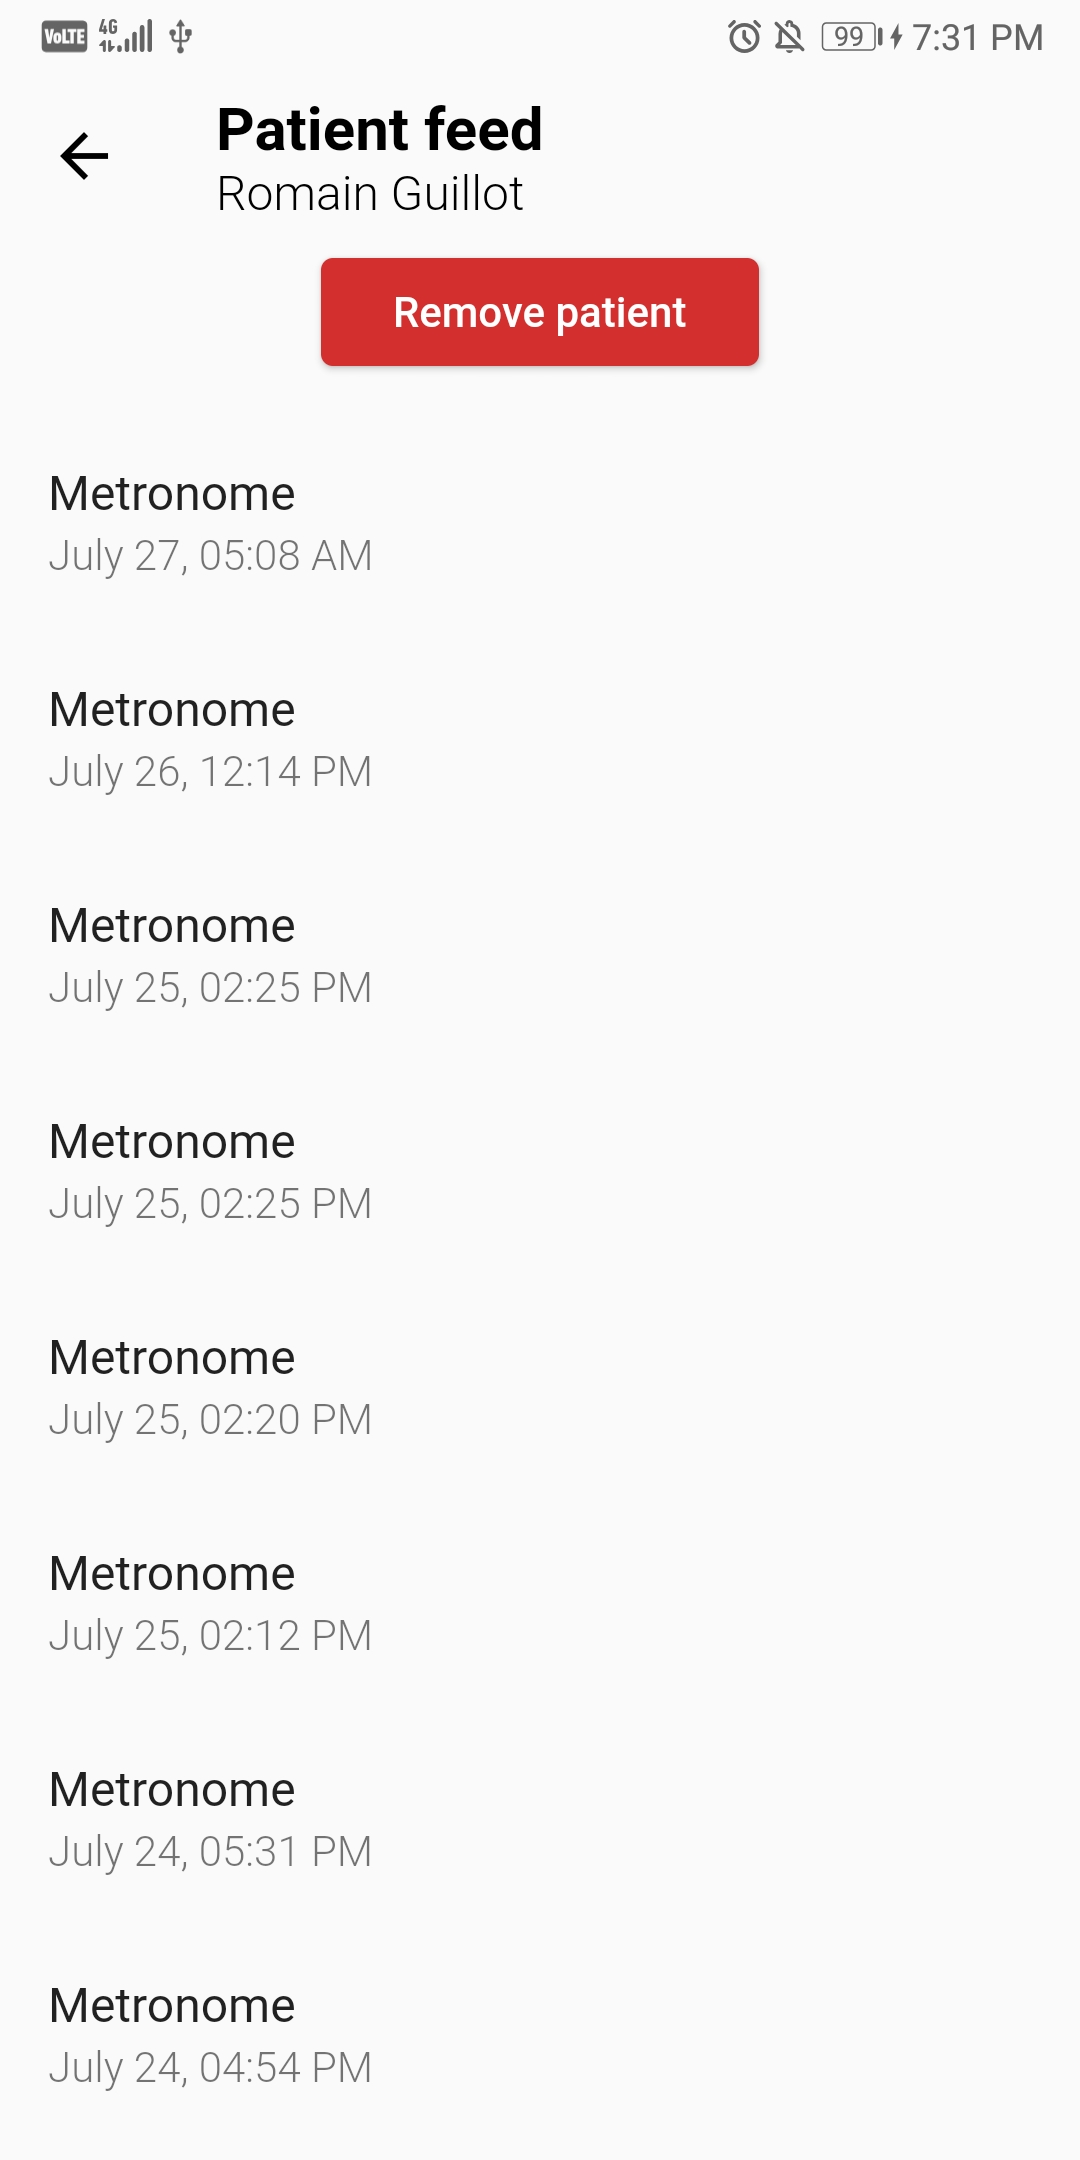
\includegraphics[width=.75\linewidth]{content/imgs/screen15.jpg}
    \caption{Progression of a patient as seen by his speech therapist}
  \end{subfigure}%
  \begin{subfigure}{.25\textwidth}
    \centering
    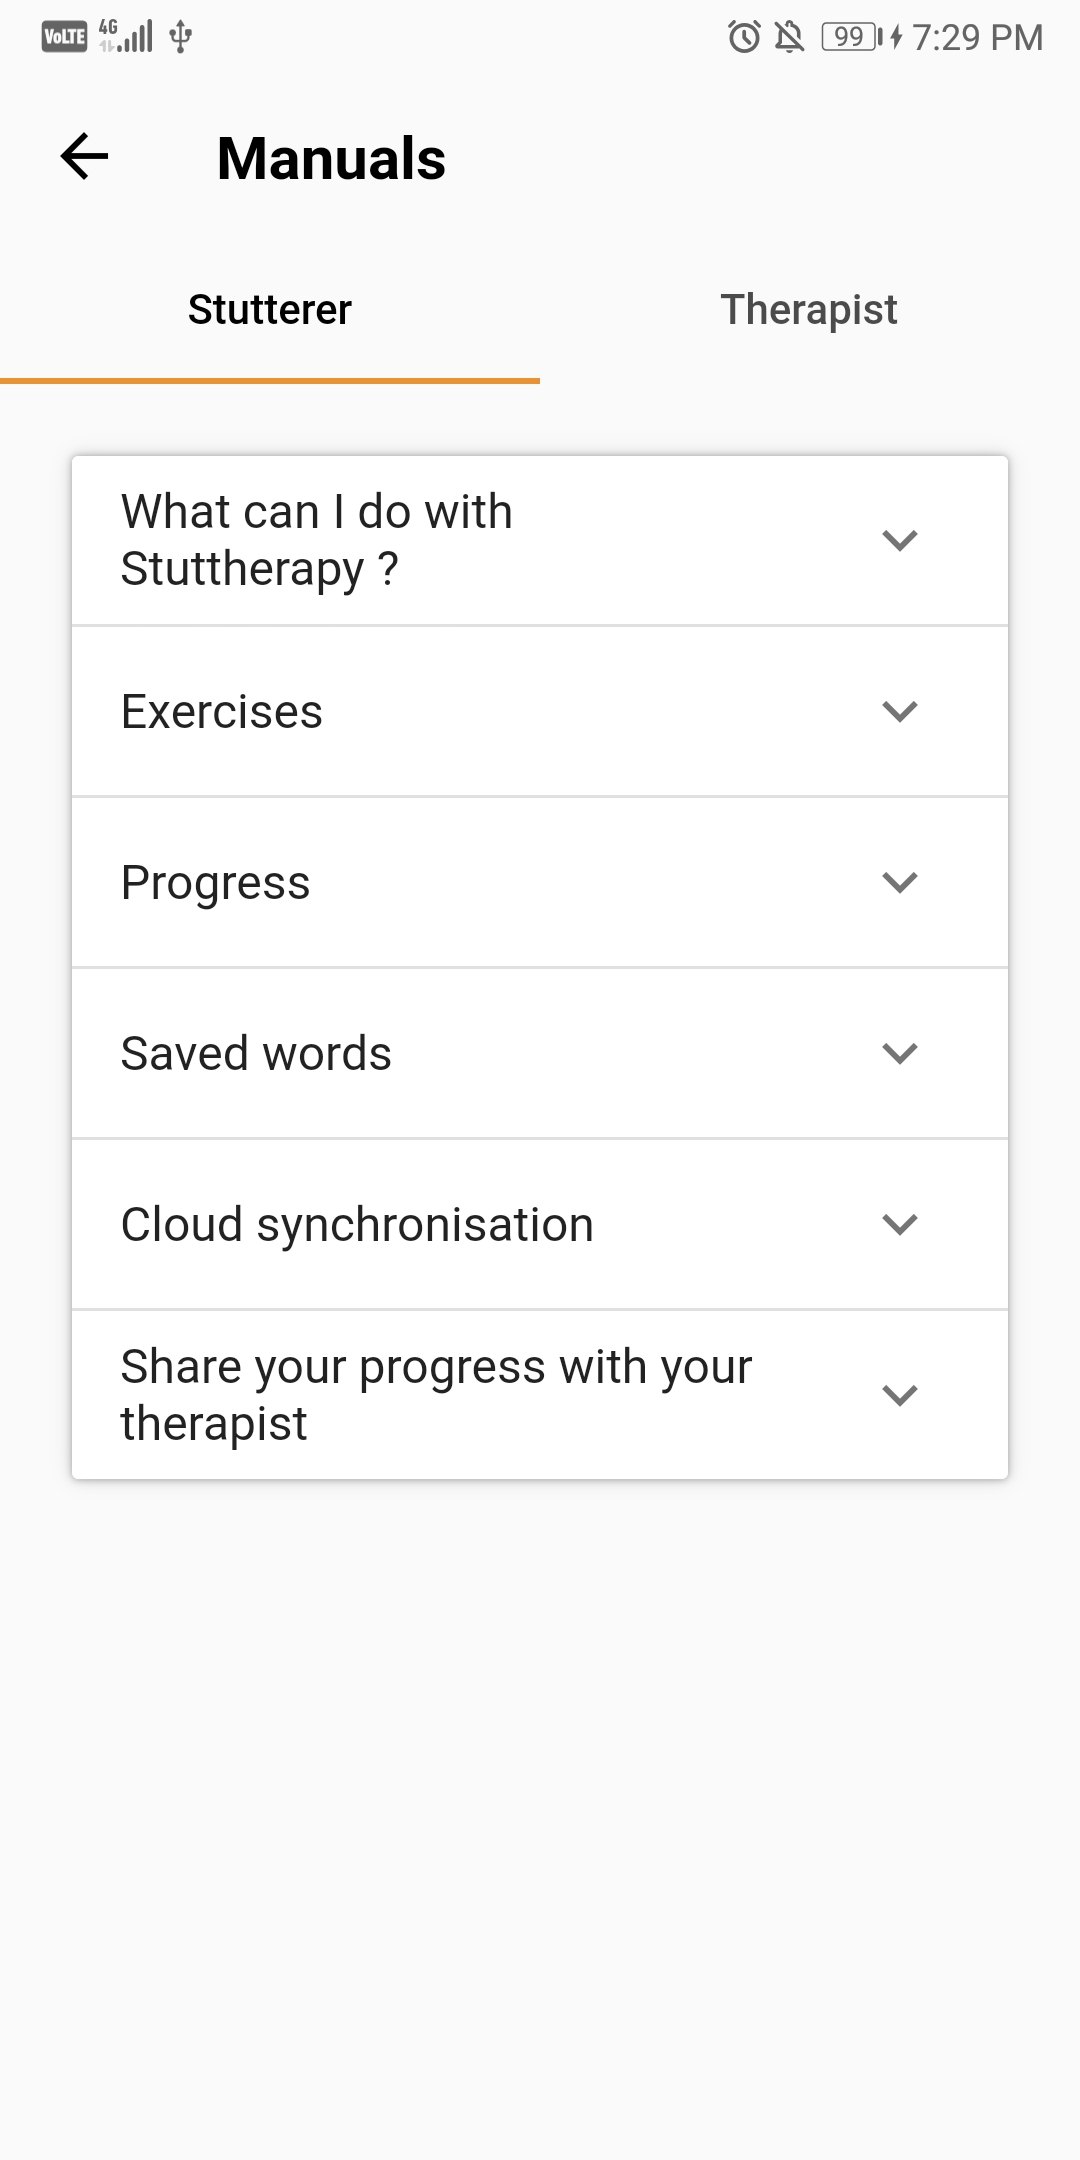
\includegraphics[width=.75\linewidth]{content/imgs/screen16.jpg}
    \caption{Guide to use the application}
  \end{subfigure}


  \caption*{Stuttherapy screenchots}
\end{figure}

\end{landscape}




\end{appendices}
